\chapter{Methodology}\label{ch:methodology}
In this chapter, we are going to discuss the proposed framework and its main components in detail. The proposed method is efficient and computationally inexpensive compared to other methods proposed in literature. 


%-------------------------------------------------------------------------
\section{Deep Learning Basics}
\subsection{Deep learning}
Machine Learning (\gls{ml}) is a field of \gls{ai} that utilizes statistical techniques to learn hidden patterns from available data and make decisions on unseen records. The core task of a \gls{ml} algorithms is to first build a general model based on the probability distribution of training examples, and then generalize its experience on unseen examples. The process of learning is highly dependent on the quality of data representation.

Deep Learning (\gls{dl}) is an advanced branch of the \gls{ml} field that aims to discover the complex representation out of simpler representations. \gls{dl} methods are typically based on artificial neural networks that consist of multiple hidden layers with nonlinear processing units. The word 'deep' refers to the multiple hidden layers that are used for transforming the data representation. Using the concept of feature learning, each hidden layer of neural networks maps its input data into a new representation. The succeeding layer tends to capture a higher level of abstraction from the less abstract concept in the preceding layer and the hierarchy of learned features in multiple levels are finally mapped to the output of the \gls{ml} task (e.g., classification and regression) in an unified framework.

Although, deep neural networks automatically extract rich and high level features which is needed for feature engineering, one of the most time-consuming parts of machine learning practice, increasing the depth does not necessarily improve their performance. Firstly, because they easily suffer from the over-fitting problem, which means the model does not generalize well to test cases. Secondly, because they are more difficult to train and more training data is needed for convergence. To alleviate this problem special types of \gls{dnn}, e.g., convolutional neural network and recurrent neural networks are introduced.

\gls{dl} architectures are divided into two broad categories: (1) unsupervised learning approaches including restricted boltzmann machines (RBMs), deep autoencoders, and generative adversarial networks (GANs), (2) supervised learning approaches including deep neural networks (\gls{dnn}s), convolutional neural networks (\gls{cnn}s), and recurrent neural networks (\gls{rnn}s).

Some of the real-world applications of Deep Learning include image recognition~\cite{Krizhevsky_12}, image captioning~\cite{Mao_15}, machine translation~\cite{kal_13}, video classification~\cite{karpathy_14} and speech recognition~\cite{graves_13}. This thesis seeks to contribute to this growing area of research by exploring the potential power of deep learning techniques in gait recognition. 


\begin{figure}
	\centering
	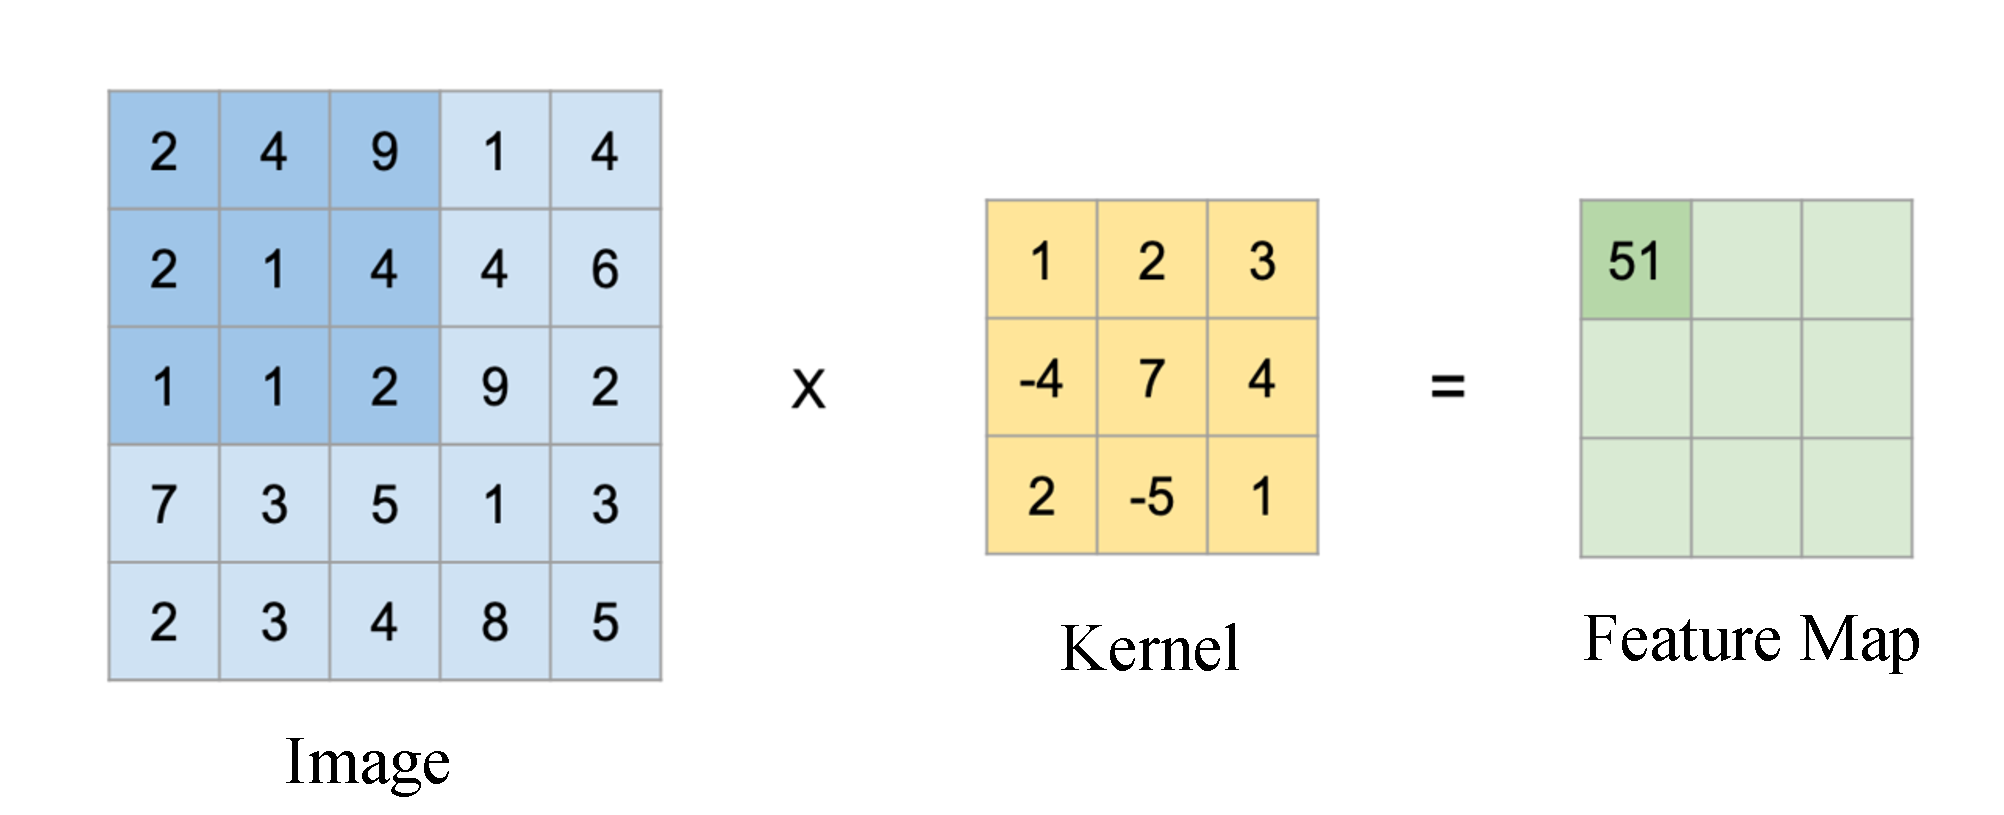
\includegraphics[width=0.8\textwidth]{figures/convolution.eps}
	\caption[Computing output activation of a convolutional layer]
	{Computing output activation of a convolutional layer \label{fig:convolution}}
\end{figure}


\subsection{Convolutional Neural Networks}
Convolutional neural networks (ConvNets or CNNs) are a category of neural networks which are proven to be very effective in areas such as image recognition~\cite{Krizhevsky_12}, video classification~\cite{karpathy_14}, action recognition~\cite{Tran_15}. They were inspired by biological processes~\cite{Hubel_68} in that the connectivity pattern between neurons resembles the organization of the animal visual cortex. Individual neurons respond to stimuli only in a restricted region of the visual field known as the \textit{receptive field}. The receptive fields of different neurons partially overlap such that they cover the entire visual field. 

When the input, e.g. images, have a local topological structure that does not depend on the specific location in the global reference system, a dense connectivity pattern might be wasteful. It is usually preferable to be able to exploit the data structure. Firstly, because adapting the connectivity pattern according to the structure of the data reduces total number of parameters and hence number of the  operations performed by the network, which consequently reduces the risk of overfitting greatly. Additionally, it also reduce the memory usage and the computation time. Secondly, constraining the connectivity pattern can have the effect of forcing the network to focus on what is important, yielding faster training and better performance.

\gls{cnn}s exploit this understanding of the data by applying the same pattern detector at every locations in the image. This is formally done through a \textit{convolution}, a signal processing operation that superimposes a pattern detector usually called a \textit{filter} or \textit{kernel} on different locations of the image and emits an activation in each position to produce a matrix of activations, typically referred to as \textit{feature map}. 

Let, $\mathbf{X}$ is a two-dimensional image and $\mathbf{W}$ is the weight matrix, also called a ’kernel’, then the convolution operation can be defined as 

\begin{equation}
(W \ast X)(i, j) = \sum_{m}\sum_{n} X(m, n) W (i - m, j - n)
\end{equation}

Intuitively, the output of the convolutional layer is formed by sliding the weight matrix over the image and computing the dot product (see Figure~\ref{fig:convolution}). In any real-world application, it would be common to apply multiple kernels at once with the same convolution hence obtaining a tensor of feature maps.




\begin{figure}
	\centering
	\includegraphics[width=0.9\textwidth]{figures/RNN_unrolled.pdf}
	\caption[A typical rolled representation of a recurrent neural network]
	{(a) A typical rolled representation of a recurrent neural network. (b) Unrolled recurrent neural network for $t$\% timesteps. [Image courtesy Chris Olah~\cite{colah_15}]\label{fig:RNN_unrolled}}
\end{figure}

\subsection{Recurrent Neural Networks} 
Recurrent neural networks (\gls{rnn}s) are a type of artificial neural networks (\gls{ann}s) where the output from the previous step is fed as input to the current step. It achieves state-of-the-art performance on various tasks in different domains that include language modeling~\cite{mikolov_12}, speech recognition~\cite{graves_13}, and machine translation~\cite{kal_13}.  

RNNs implement feedback loops (see Figure~\ref{fig:RNN_unrolled}(a)) that propagate some information from one timestep to the next. It might not be immediately obvious what it means in practice to put a loop in an \gls{ann} and how to backpropagate through it. To better comprehend how RNNs work it is useful to consider its behavior explicitly by \emph{unrolling} the RNN, as shown in Figure~\ref{fig:RNN_unrolled}(b).



\begin{figure}
	\centering
	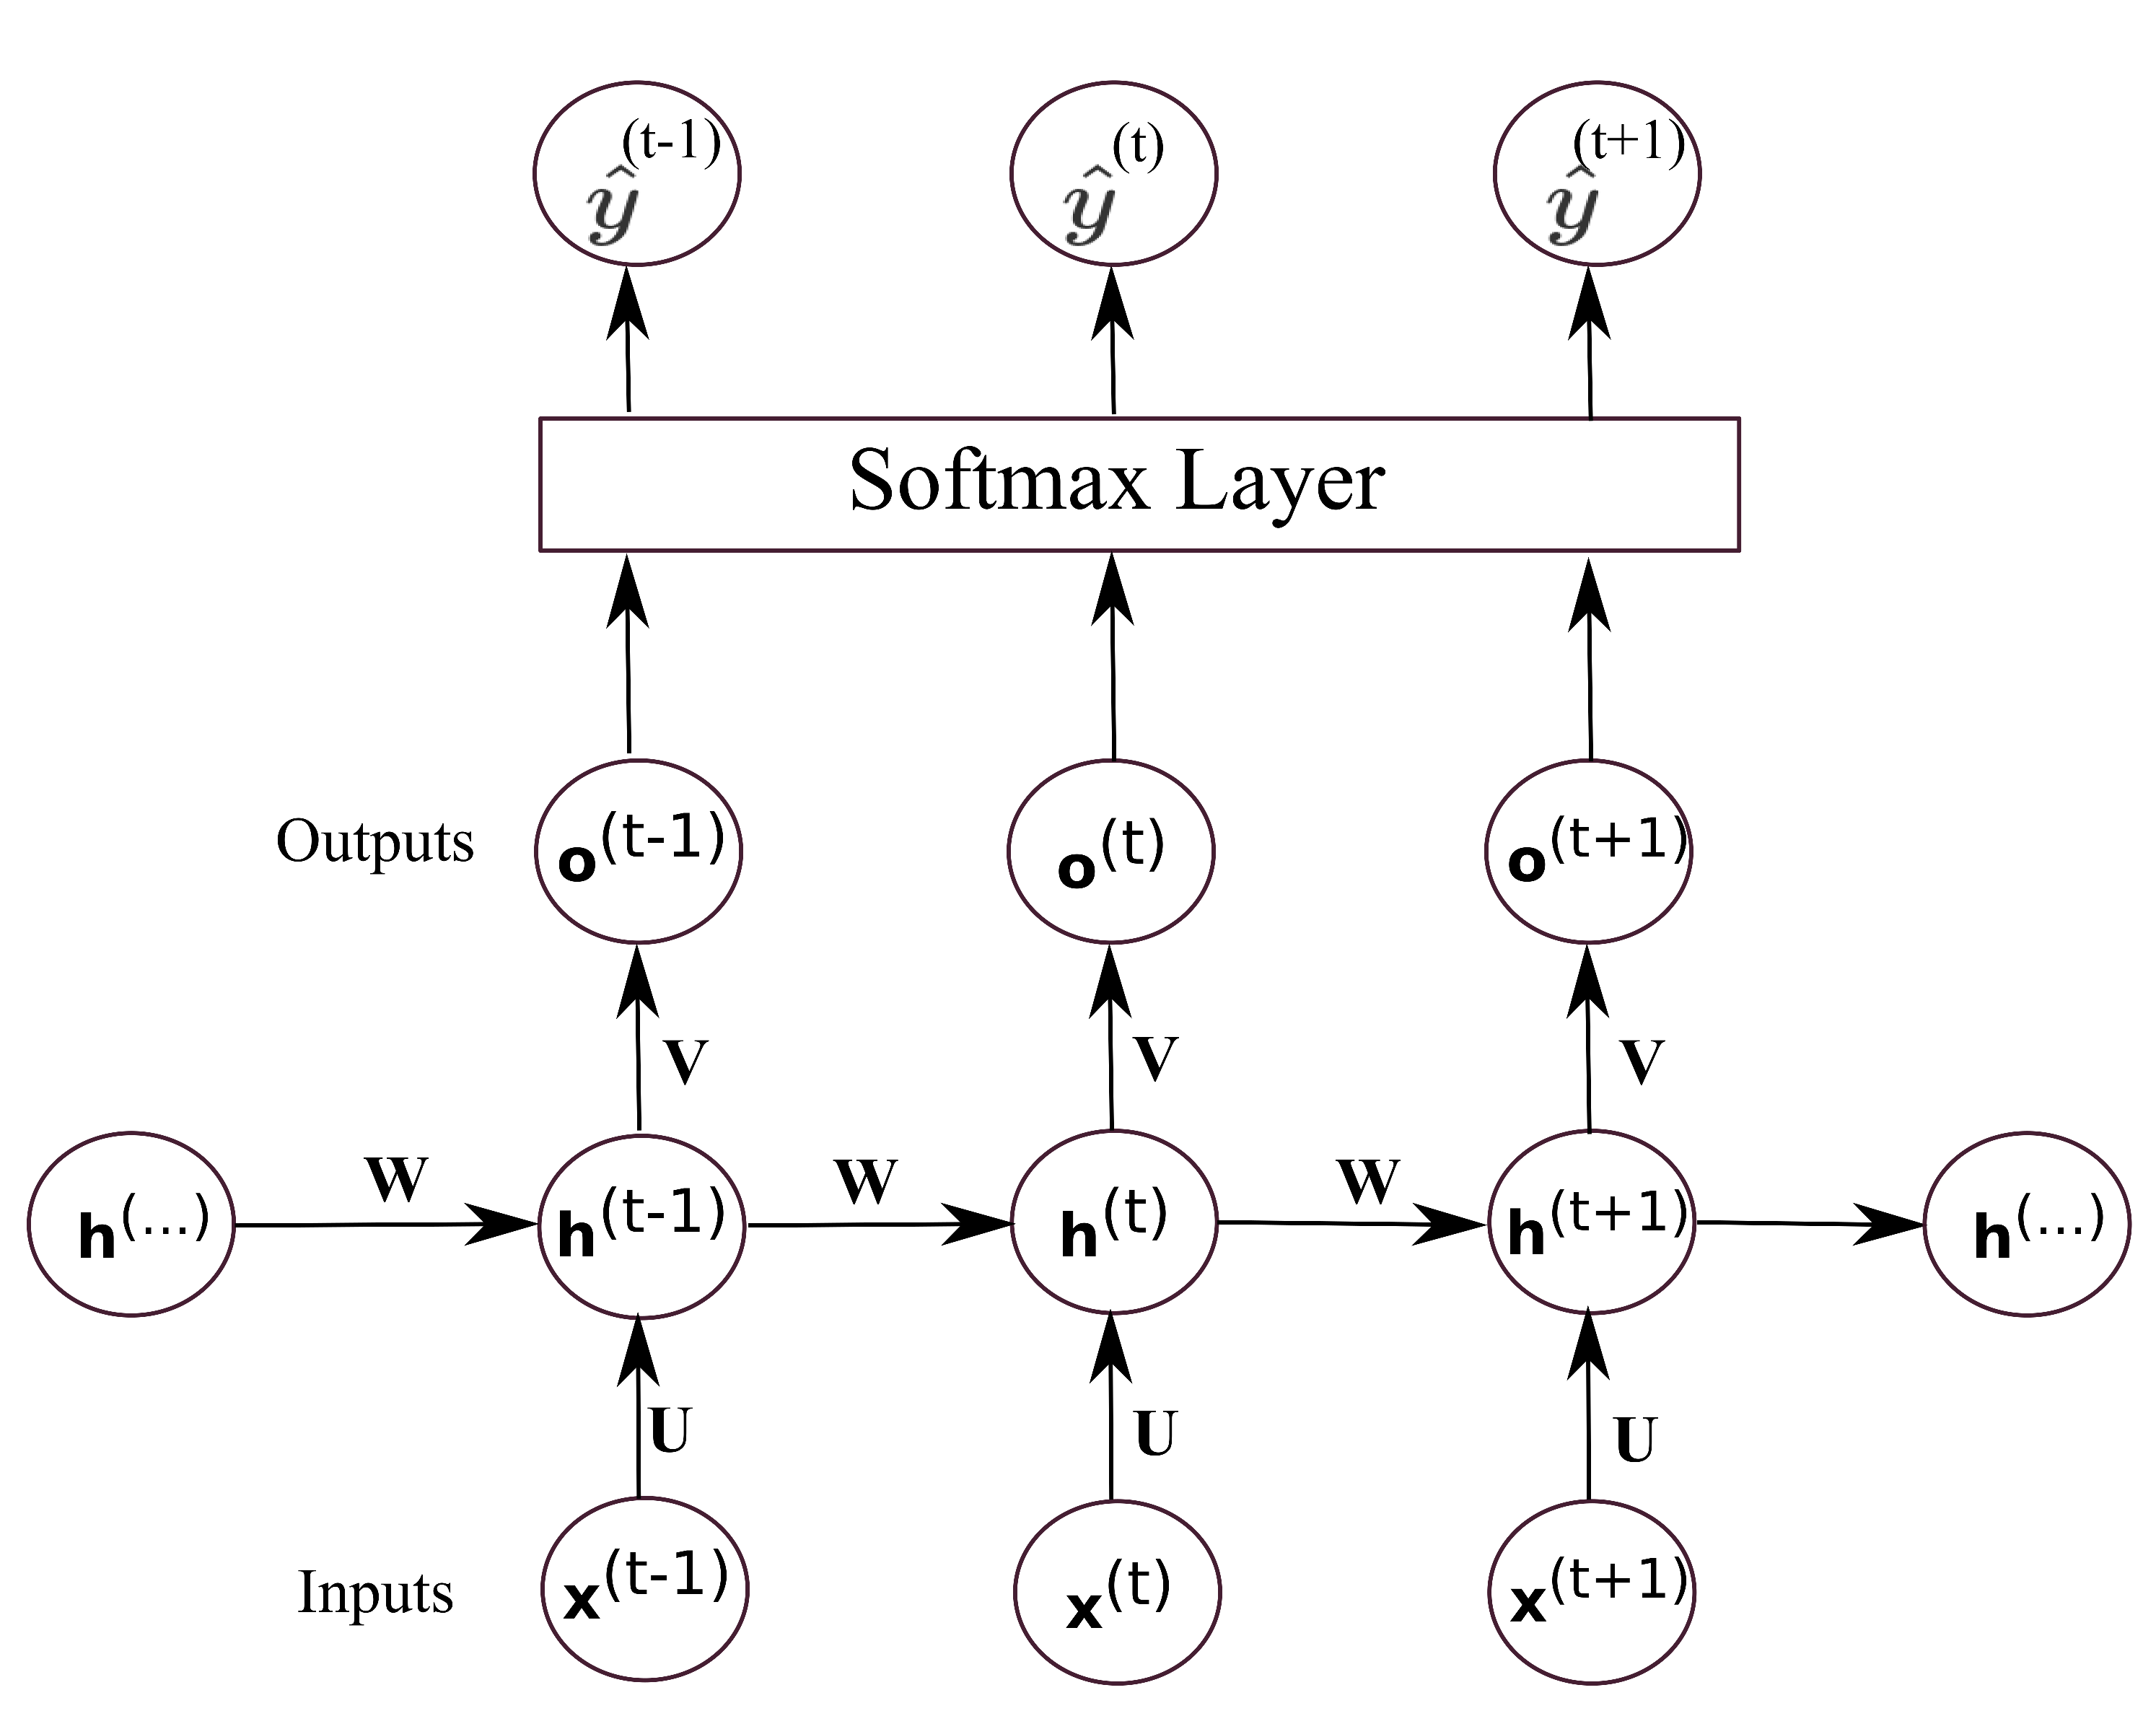
\includegraphics[width=0.8\textwidth]{figures/rnn_unrolling.eps}
	\caption{The computational graph of a unrolled recurrent network that maps an input sequence of $ x $ values to a corresponding sequence of output $ o $ values \label{fig:RNN_unrolling}}
\end{figure}

The forward propagation equations for the \gls{rnn} depicted in Figure~\ref{fig:RNN_unrolling}. Forward propagation begins with a specification of the initial state $ \textbf{h}^{(0)} $. Then, for each timestep from $ t $ we apply the following update equations:

\begin{equation} \label{rnn_unroll}
\begin{split}
	\textbf{a}^{(t)} &= \textbf{b} + \textbf{W}\textbf{h}^{(t-1)} + \textbf{U}\textbf{x}^{(t)} \\
	\textbf{h}^{(t)}&=\tanh(\textbf{a}^{(t)})\\
	\textbf{o}^{(t)}&= \textbf{c} + \textbf{V}\textbf{h}^{(t)} \\
	{\hat{\textbf{y}}}^{(t)} &= softmax(\textbf{o}^{(t)})
\end{split}
\end{equation}

Here, the parameters are the bias vectors $ \textbf{b} $ and $ \textbf{c} $ along with the weight matrices $\textbf{U}$, $\textbf{V}$ and $\textbf{W}$, respectively, for input-to-hidden, hidden-to-output and hidden-to-hidden connections. The activation of an RNN (see Figure ~\ref{fig:RNN_unrolling}) at time $t$ depends on the input at time $t$ as well as on the information coming from the previous step $t-1$. \gls{rnn}s have a very simple internal structure, that usually amounts to applying some affine transformation to the input and to the previous output, and computing some non-linearity (typically a $tanh$) of their sum.

That sequential information is preserved in the recurrent network's hidden state, which manages to span many timesteps as it cascades forward to affect the processing of each new example. It is finding correlations between events separated by many moments, and these correlations are called \textit{long-term dependencies}, because an event downstream in time depends upon, and is a function of, one or more events that came before. One way to think about RNNs is that they applies the same model to each timestep of the sequence or, equivalently, applies different models at each timestep which share their weights. 

For training these networks, it is required to unroll the computation graph and use the backpropagation algorithm to proceed from the most recent timestep, backward in time. This algorithm is usually referred to as \emph{Backpropagation through time} (\gls{bptt}). The problem of \gls{bptt} is that it requires the application of the chain rule all the way from the current timestep to $t = 0$ to propagate the gradients.  This results in a long chain of products that can easily go to infinity or become zero if the elements of the multiplication are greater or smaller than $1$ respectively ~\cite{Bengio_94}. These two issues, i.e., going to infinity and becoming zero, are known in the literature as \emph{exploding gradient} and \emph{vanishing gradient}~\cite{Hochreiter_01} problem respectively. The first one can be partially addressed by \emph{clipping the gradient} when it becomes too large, but the second is not easy to overcome and can make training these kind of models very hard.


\subsection{Long Short-Term Memory}
\begin{figure}[t]
	\centering
	\includegraphics[width=0.7\textwidth]{figures/LSTM.pdf}
	\caption[A Long Short Term Memory (LSTM)]
	{A Long Short Term Memory (LSTM). [Image courtesy Chris Olah~\cite{colah_15}]\label{fig:LSTM}}
\end{figure}

Long short-term memory (\gls{lstm}) networks (Figure~\ref{fig:LSTM}) have been proposed to solve the problems of RNNs in modeling long-term dependencies. LSTMs have been designed to have an internal memory, or~\emph{state}, that can be updated at each timestep. As opposed to vanilla \gls{rnn}, this internal memory allows LSTM to separate their output from the information they want to carry over into the future steps.

\begin{figure}[t]
	\centering
	\includegraphics[width=0.6\textwidth]{figures/LSTM_state.pdf}
	\caption[The internal state of LSTMs]
	{The internal state of LSTMs. [Image courtesy Chris Olah~\cite{colah_15}]\label{fig:LSTM_state}}
\end{figure}

Figure \ref{fig:LSTM_state} highlights the internal memory path. From the figure it can be observed that how the internal memory of the previous timestep $\mathbf{c}_{t-1}$ is carried over to the current timestep where it is updated through a multiplicative and an additive interaction and concurs to determine the current state of the memory $\mathbf{c}_t$. Thereafter, this state once again, propagated to the next timestep.


\begin{figure}[p]
	\centering
	\includegraphics[width=0.6\textwidth]{figures/LSTM_forget_gate.pdf}
	\caption[The LSTM forget gate]
	{The LSTM forget gate. [Image courtesy Chris Olah~\cite{colah_15}]\label{fig:LSTM_forget_gate}}
\end{figure}
\begin{figure}[p]
	\centering
	\includegraphics[width=0.6\textwidth]{figures/LSTM_input_gate.pdf}
	\caption[The LSTM input gate]
	{The LSTM input gate. [Image courtesy Chris Olah~\cite{colah_15}]\label{fig:LSTM_input_gate}}
\end{figure}
\begin{figure}[p]
	\centering
	\includegraphics[width=0.6\textwidth]{figures/LSTM_output_gate.pdf}
	\caption[The LSTM output gate]
	{The LSTM output gate.[Image courtesy Chris Olah~\cite{colah_15}]\label{fig:LSTM_output_gate}}
\end{figure}

\gls{lstm}s interact with memory through \emph{gate}, a computational node, that determines the behavior of the model. The \emph{forget~gate}, as shown in Figure~\ref{fig:LSTM_forget_gate}, determines how much of the previous step's memory to forget or, equivalently, how much of the previous state to retain.  This is modeled through a sigmoid layer ($\sigma$) that takes the current input $\mathbf{x}_t$ and the output of the previous step $\mathbf{h}_{t-1}$ and produces an activation vector between $0$ and $1$.  This activation is multiplied by the previous state $\mathbf{c}_{t-1}$ and results in an intermediate memory state where some of the activations can be weaker than those in $\mathbf{c}_{t-1}$ and some others are potentially zeroed out.

The forget gate allows the LSTM to discard information that is not relevant anymore. 
\begin{equation}\label{eq:LSTM_forget_gate}
\mathbf{f}_t = \sigma\left(\mathbf{W}_f \cdot \mathbf{x}_t + \mathbf{U}_f \cdot \mathbf{h}_{t-1} + \mathbf{b}_f \right),
\end{equation}

Again, \gls{lstm}s have a mechanism to add new information to the memory. This behavior is controlled by an \emph{input gate} (Figure \ref{fig:LSTM_input_gate}) that modulates the amount of the current input that is going to be stored in the memory. This operation is split over two computation paths: similarly to the forget gate, the input gate takes the current input $\mathbf{x}_t$ and the output of the previous step $\mathbf{h}_{t-1}$ and exploits a sigmoid layer to produce an activation vector between $0$ and $1$. Simultaneously, a $tanh$ layer generates a state update $\mathbf{\tilde c}_t$ between $-1$ and $1$. This is governed by the following equations:

\begin{equation}\label{eq:LSTM_input_gate}
\begin{split}
\mathbf{i}_t &= \sigma\left(\mathbf{W}_i \cdot \mathbf{x}_t + \mathbf{U}_i \cdot \mathbf{h}_{t-1} + \mathbf{b}_i \right)\\
\mathbf{\tilde c}_t &= tanh \left(\mathbf{W}_c \cdot \mathbf{x}_t + \mathbf{U}_c \cdot \mathbf{h}_{t-1} + \mathbf{b}_c \right)
\end{split}
\end{equation}

The input gate modulates how much of this state update will be applied to the old state to generate the current state. The forget gate $\mathbf{f}_t$ and the input gate $\mathbf{i}_t$, together with the state update $\mathbf{\tilde c}_t$ and the previous state $\mathbf{c}_{t-1}$ fully determine the state at time $t$. 

\begin{equation}\label{eq:LSTM_state_update}
\mathbf{c}_t = \mathbf{f}_t \circ \mathbf{c}_{t-1} + \mathbf{i}_t \circ \mathbf{\tilde c}_t
\end{equation}

The last gate of \gls{lstm} is the \emph{output~gate} (Figure~\ref{fig:LSTM_output_gate}) $\mathbf{o}_t$ that, as the name reveals, manipulates the output of the LSTM at time $t$. The usual sigmoid layer determines the state of the output gate and the memory resulting from the transformations due to the forget and input gates goes through a $tanh$ nonlinearity and is multiplied by the output gate to finally produce the output.

\begin{equation}\label{eq:LSTM_output_gate}
\begin{split}
\mathbf{o}_t &= \sigma\left(\mathbf{W}_o \cdot \mathbf{x}_t + \mathbf{U}_o \cdot \mathbf{h}_{t-1} + \mathbf{b}_o \right)\\
\mathbf{h}_t &= \mathbf{o}_t \circ tanh \left(\mathbf{c}_t\right)
\end{split}
\end{equation}


\begin{figure}
	\centering
	\includegraphics[width=0.6\textwidth]{figures/GRU.pdf}
	\caption[Gated Recurrent Units (GRUs)]
	{Gated Recurrent Units (GRUs). [Image courtesy Chris Olah~\cite{colah_15}]\label{fig:GRU}}
\end{figure}

\subsection{Gated Recurrent Unit}\label{sec:GRU}
Cho \textit{et al.}~\cite{Cho_14} proposed a new kind of RNN called gated recurrent unit (\gls{gru}), as shown in Figure~\ref{fig:GRU}, with less gates than \gls{lstm} and a different internal structure. In \gls{gru}s the forget and input gates are coupled into an~\emph{update gate} $\mathbf{z}_t$.  The memory and output are also merged into a single state and the internal structure is modified to cope with these changes. Figure~\ref{fig:GRU} shows the internal structure of a GRU unit.

The \textit{update gate} $\mathbf{z}_t$ for timestep $t$ helps the model to determine how much of the information from the previous timestep needs to be passed along the future.  It is analogous to the output gate in an LSTM cell.
\begin{equation}
\mathbf{z}_t = \sigma \left(\mathbf{W}_z \cdot \mathbf{x}_t + \mathbf{U}_z \cdot \mathbf{h}_{t-1} + \mathbf{b}_z\right)
\end{equation}

On the other hand, \textit{reset gate} in GRU is used to decide how much of the past information needs to forget. It is analogous to the combination of the input Gate and the forget Gate in an LSTM cell.
\begin{equation}
\mathbf{r}_t = \sigma \left(\mathbf{W}_r \cdot \mathbf{x}_t + \mathbf{U}_r \cdot \mathbf{h}_{t-1} + \mathbf{b}_r\right)
\end{equation}

GRU has also a new memory content will use the reset gate to store the relevant information from the past
\begin{equation}
\mathbf{\tilde h}_t = tanh \left(\mathbf{W}_h \cdot \mathbf{x}_t + \mathbf{U}_h \cdot (\mathbf{r}_t \circ \mathbf{h}_{t-1}) + \mathbf{b}_h\right)
\end{equation}

In the last step, the GRU calculate the current information $\mathbf{h}_t$ from update gate ($\mathbf{z}_t$), previous information ($\mathbf{h}_{t-1}$) and memory content ($\mathbf{\tilde h}_t$) and passes it down to the network. 
\begin{equation}
\mathbf{h}_t = \mathbf{z}_t \circ \mathbf{h}_{t-1} + (1 - \mathbf{z}_t) \circ \mathbf{\tilde h}_t.
\end{equation}

Therefore, the differences between LSTM unit and GRU are:
\begin{itemize}
	\item GRUs have 2 gates while LSTMs have 3 gates
	\item GRUs do not have any internal memory in contrast to LSTMs
	\item Nonlinearity is not applied when computing the output of GRUs
\end{itemize}

The advantage of \gls{gru}s over \gls{lstm}s is the smaller number of gates that make them less memory as well as computationally intense, which is often a critical aspect for \gls{ann}s. Therefore, GRU involves less computation compared with LSTM while keeping similar performance and improving the efficiency of the original \gls{rnn}s. Moreover, \gls{gru} has shown better classification performance on smaller datasets~\cite{Chung_14}.

\begin{figure}[t]
	\centering
	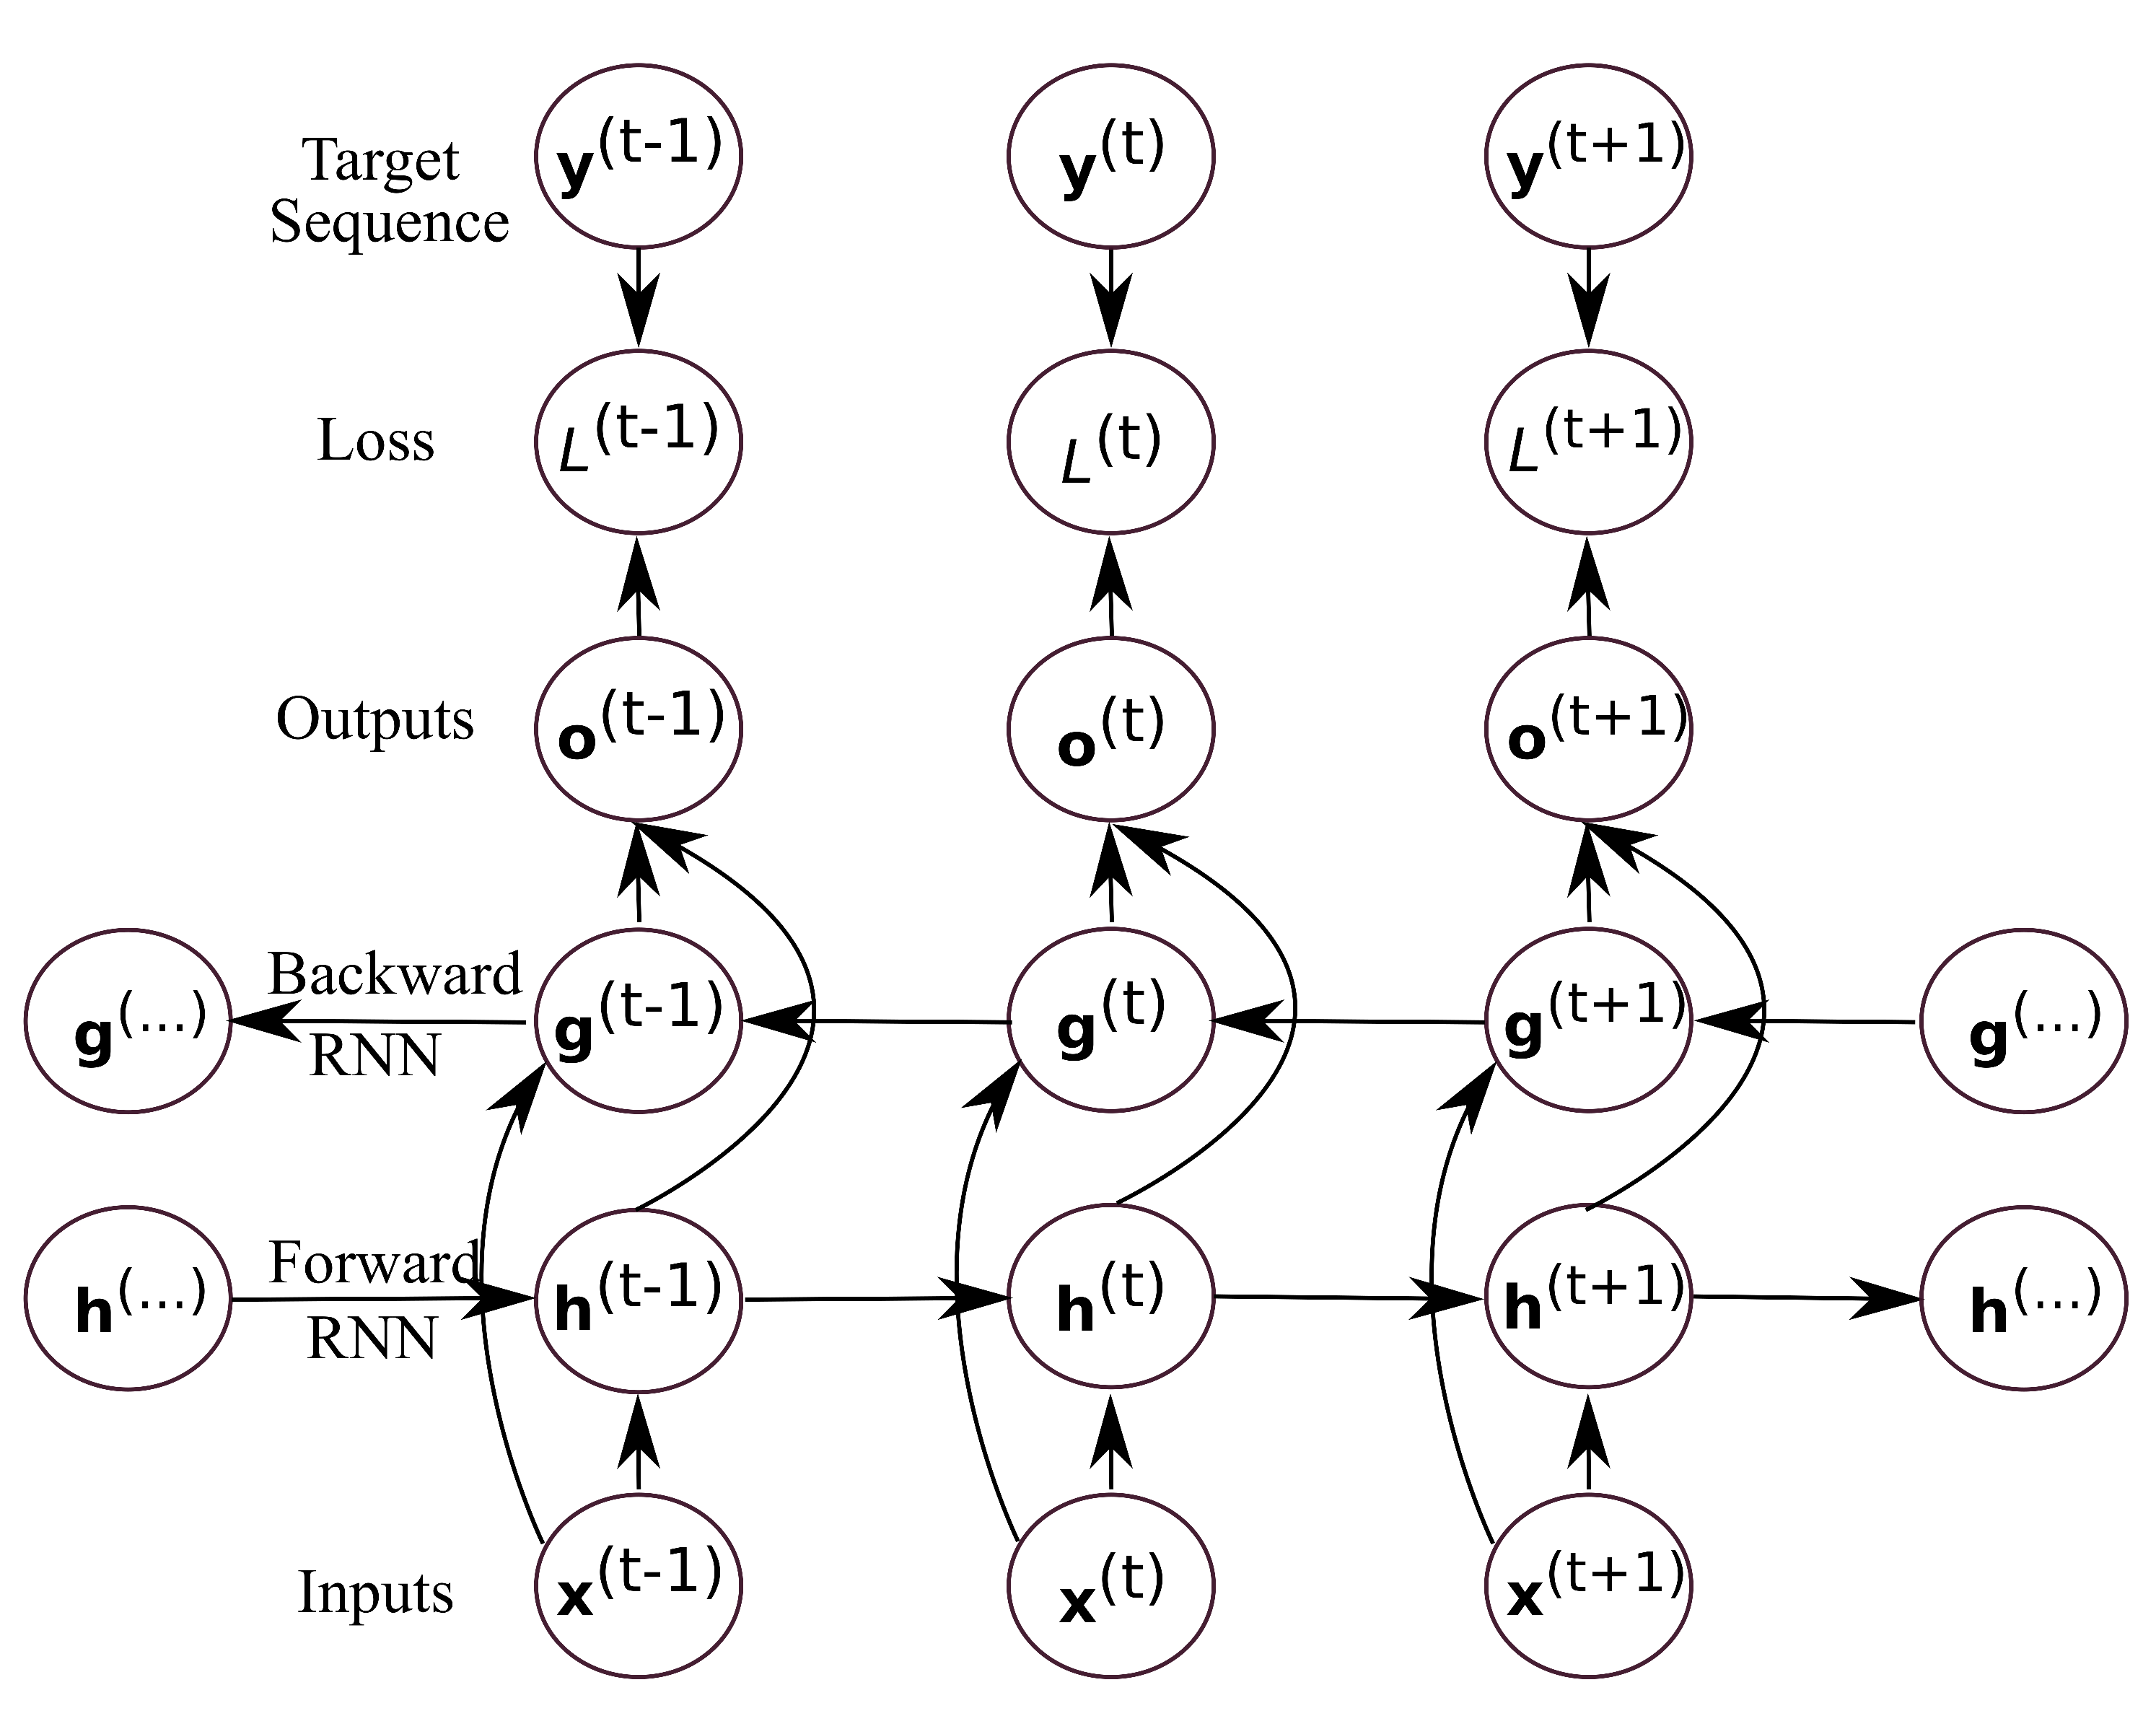
\includegraphics[width=0.9\textwidth]{figures/brnn.eps}
	\caption{The architecture of a vanilla bidirectional recurrent neural network \label{fig:bidirectional_rnn}}
\end{figure}



\subsection{Bidirectional RNNs}
Bidirectional recurrent neural networks (\gls{brnn}s)~\cite{Schuster_97} connect two hidden layers running in opposite directions to a single output, allowing them to receive information from both past and future states. Here, the input sequence is fed in normal time order for one network, and in reverse time order for another. The outputs of the two networks are usually concatenated at each timestep. So, this type of structure allows the networks to have both backward and forward information about the sequence at every timestep. \gls{brnn} are especially useful when the context of the input is needed. For example, in handwriting recognition~\cite{Graves_08}, the performance can be enhanced by knowledge of the letters located before and after the current letter.  A vanilla architecture of the \gls{brnn} is illustrated in Figure~\ref{fig:bidirectional_rnn}. 


\subsubsection{Bidirectional GRU}
In a  bidirectional GRU (\gls{bigru}) consists of 2 vanilla unidirectional \gls{gru}s stacked side by side, but the second GRU reads the input sequence from the opposite direction. Figure~\ref{fig:bidirectional_gru} illustrates the basic architecture of a Bidirectional GRU. 
\begin{figure}[t]
	\centering
	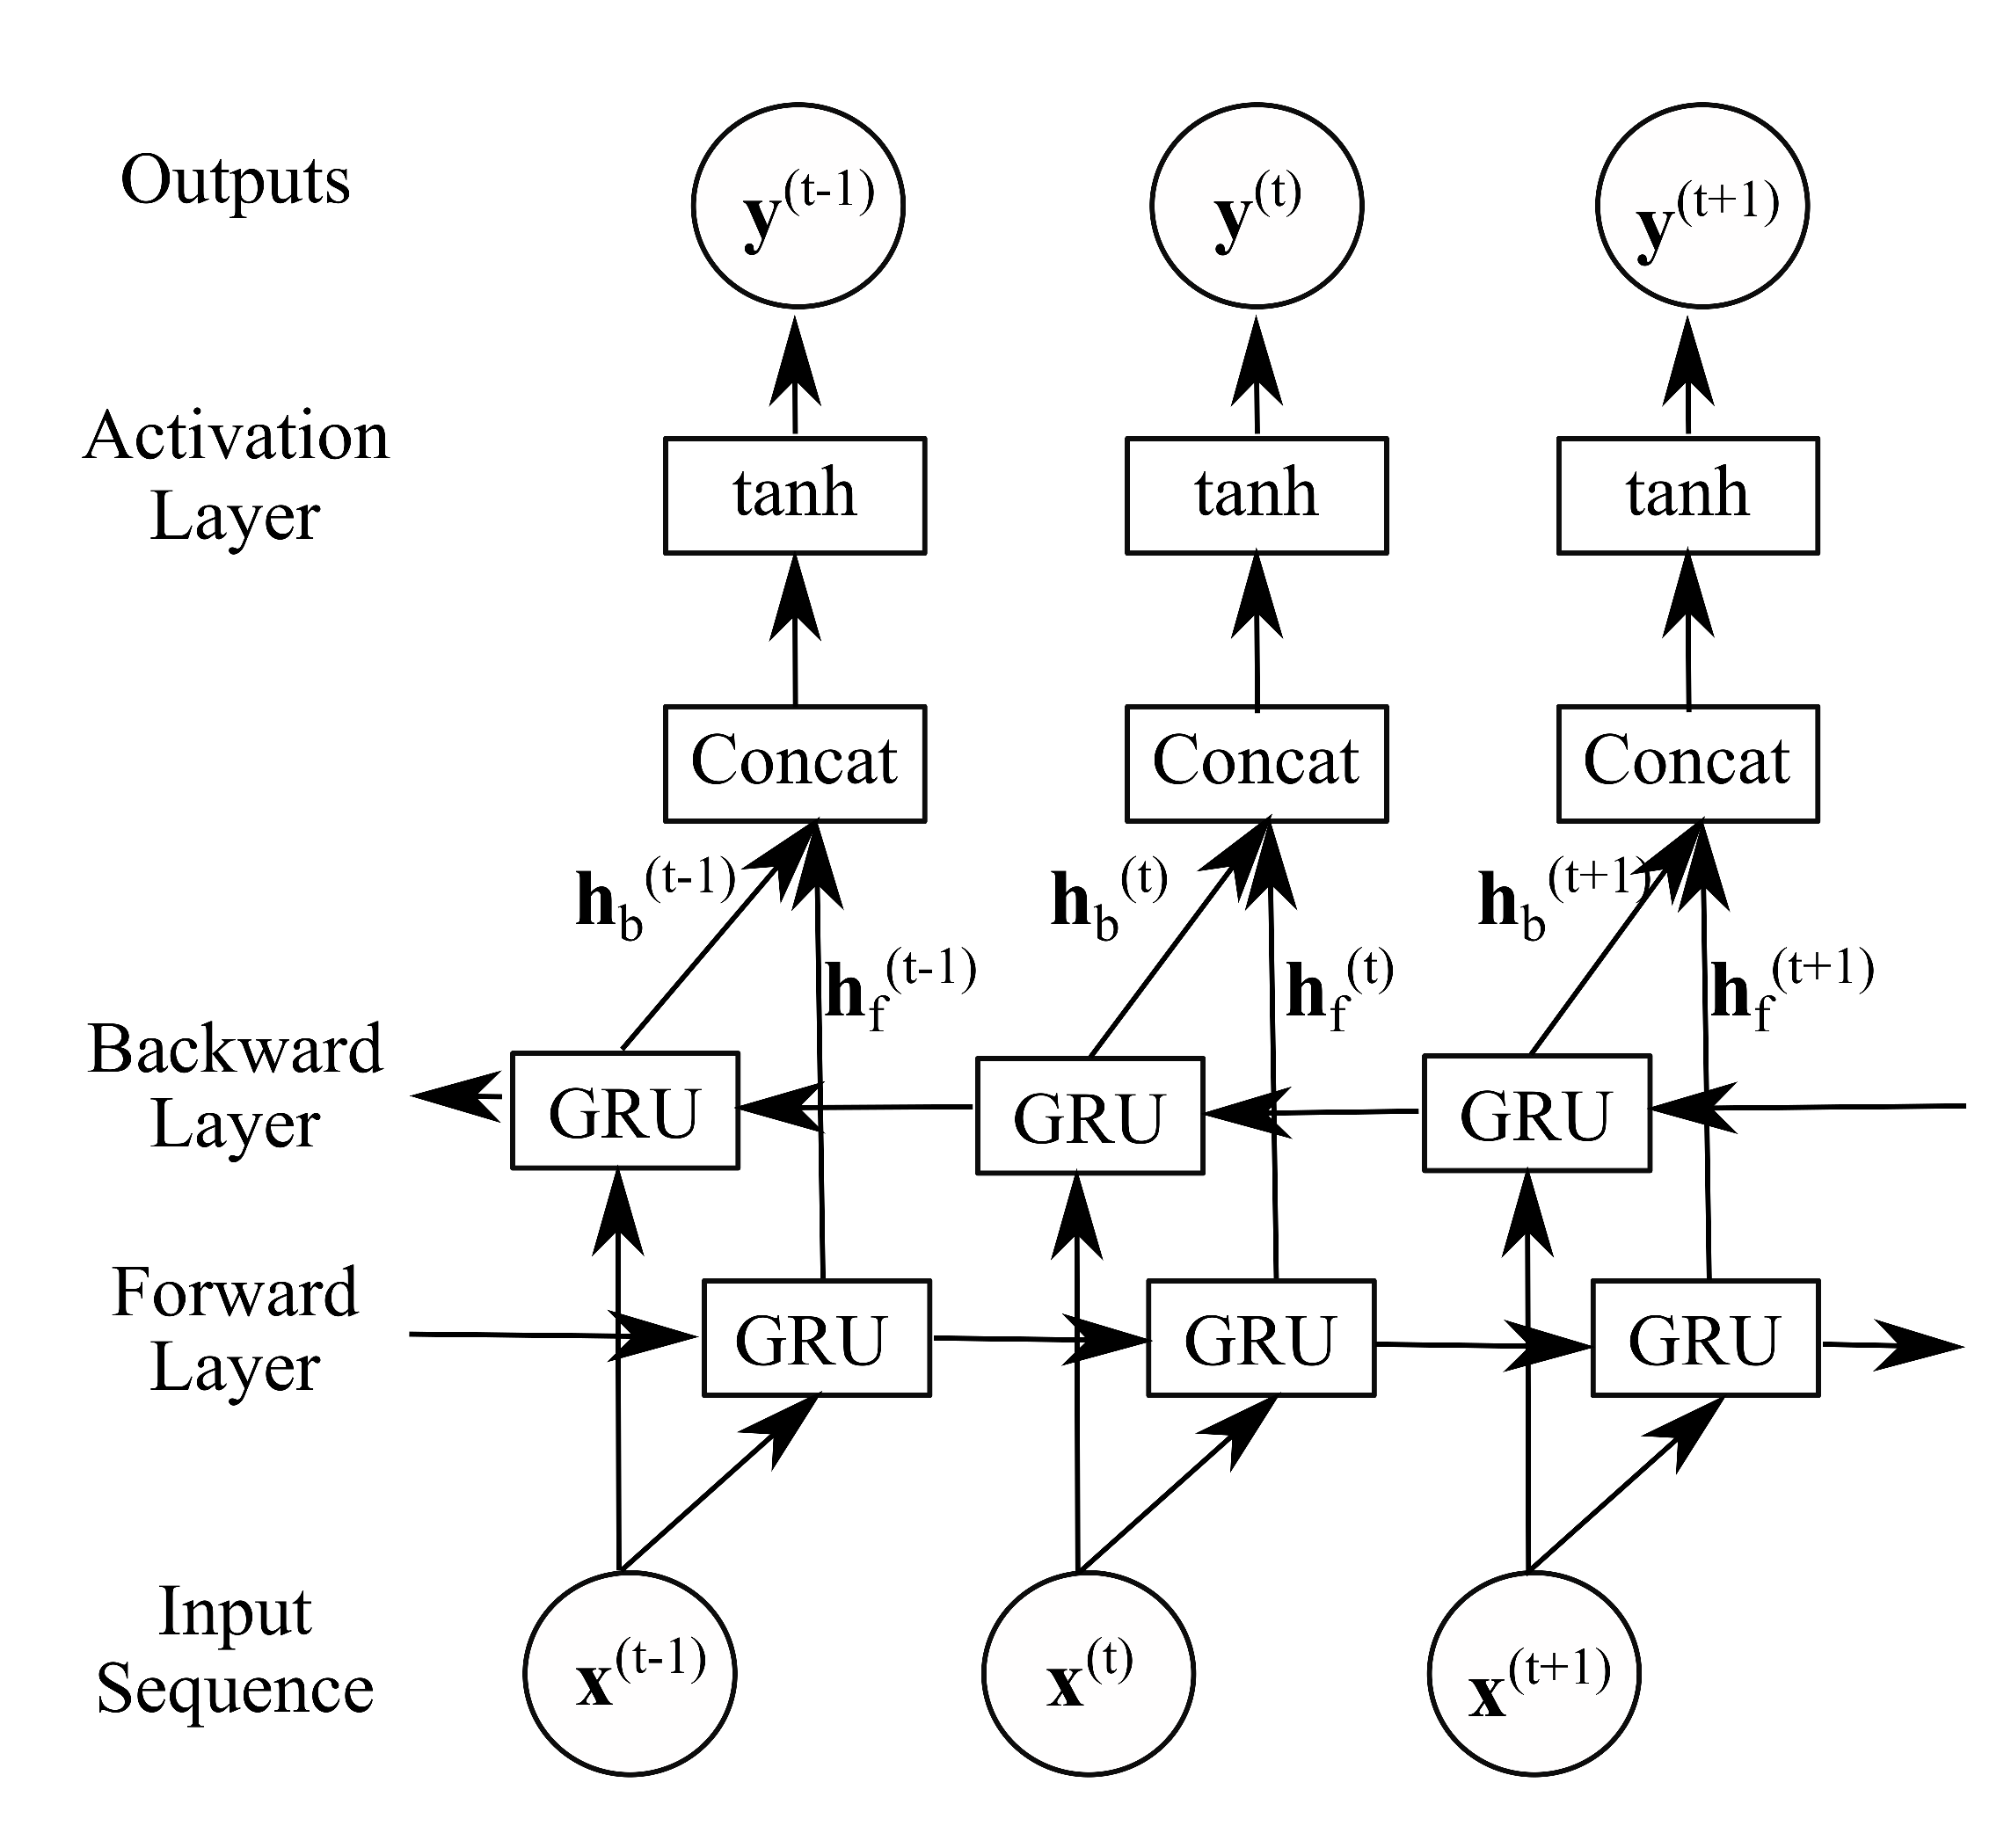
\includegraphics[width=0.7\textwidth]{figures/bigru.eps}
	\caption{The architecture of a bidirectional gated recurrent neural network \label{fig:bidirectional_gru}}
\end{figure}


\subsection{Regularization for Deep Learning}
Regularization is a technique which makes slight modifications to the learning algorithm such that the model generalizes better. This in turn improves the model's performance on the test data. As we know, \gls{dnn}s are highly complex models (many parameters and many non-linearities) and they are easy to overfit, hence, we need some form of regularization. 

\subsubsection{L2 Regularization}
This regularization is popularly known as \textit{weight decay}. This strategy drives the weights closer to the origin by adding the regularization term. This technique is also known as \textit{ridge regression}.

\subsubsection{Dropout}
Dropout is a computationally inexpensive but powerful regularization method.

One advantage of dropout is that it is very computationally cheap. Using dropout during training requires only $ O(n) $ computation per example per update, to generate n random binary numbers and multiply them by the state. Another significant advantage of dropout is that it does not significantly limit the type of model or training procedure that can be used. It works well with nearly any model that uses a distributed representation and can be trained with stochastic gradient descent.


\subsubsection{Dataset Augmentation}
The simplest way to reduce overfitting is to increase the size of the training data. But mostly we are provided with limited data. One way is to create fake data and add it to our training dataset, for some domains this is fairly straightforward and easy.

\subsubsection{Early Stopping of Training}
One way to think of early stopping is as a very efficient hyperparameter selection algorithm. The idea of early stopping of training is that as soon as the validation error starts to increase we freeze the parameters and stop the training process. Or we can also store the copy of model parameters every time the error on the validation set improves and return these parameters when the training terminates rather than the latest parameters.

Early stopping has an advantage over weight decay that early stopping automatically determines the correct amount of regularization while weight decay requires many training experiments with different values of its hyperparameter.


\subsubsection{Noise Robustness}
Noise is often introduced to the inputs as a dataset augmentation strategy. the addition of noise with infinitesimal variance at the input of the model is equivalent to imposing a penalty on the norm of the weights. Noise injection is much more powerful than simply shrinking the parameters, especially when the noise is added to the hidden units.

Another way that noise has been used in the service of regularizing models is by adding it to the weights. This technique has been used primarily in the context of recurrent neural networks. This can be interpreted as a stochastic implementation of Bayesian inference over the weights.


\section{Human Pose Estimation}
Human pose estimation, one of the core problems in computer vision, refers to the process of inferring poses in an image or video. Essentially, it entails predicting the body parts or body joint positions of individuals in an image.
It is the key component which enables machines to have a perception of the people in images and videos. It has been successfully employed in many real-world applications such as action recognition~\cite{Song_17}, augmented reality~\cite{Marchand_16}, gaming~\cite{Ke_10}, and gait recognition~\cite{Liao_19}. 


\subsection{Types of Pose Estimation} 
Depending upon the output dimension requirement, a pose estimation algorithm can be categorized into 2D pose estimation and 3D pose estimation. In 2D pose estimation, the location of body joint is predicted in terms of pixel values of the image frame. On the other hand, 3D pose estimation is predicting a three-dimensional spatial arrangement of all the body joints as its final output. Again, depending on the number of people being tracked, pose estimation can be further classified into single-person and multi-person. Single-person pose estimation guarantees of only one person present in the frame, whereas, in multi-person pose estimation, each image may contain an unknown number of people who can appear at any position or scale. Therefore, it needs to handle the additional problem of inter-person occlusion. 

\begin{figure}[t]
	\centering
	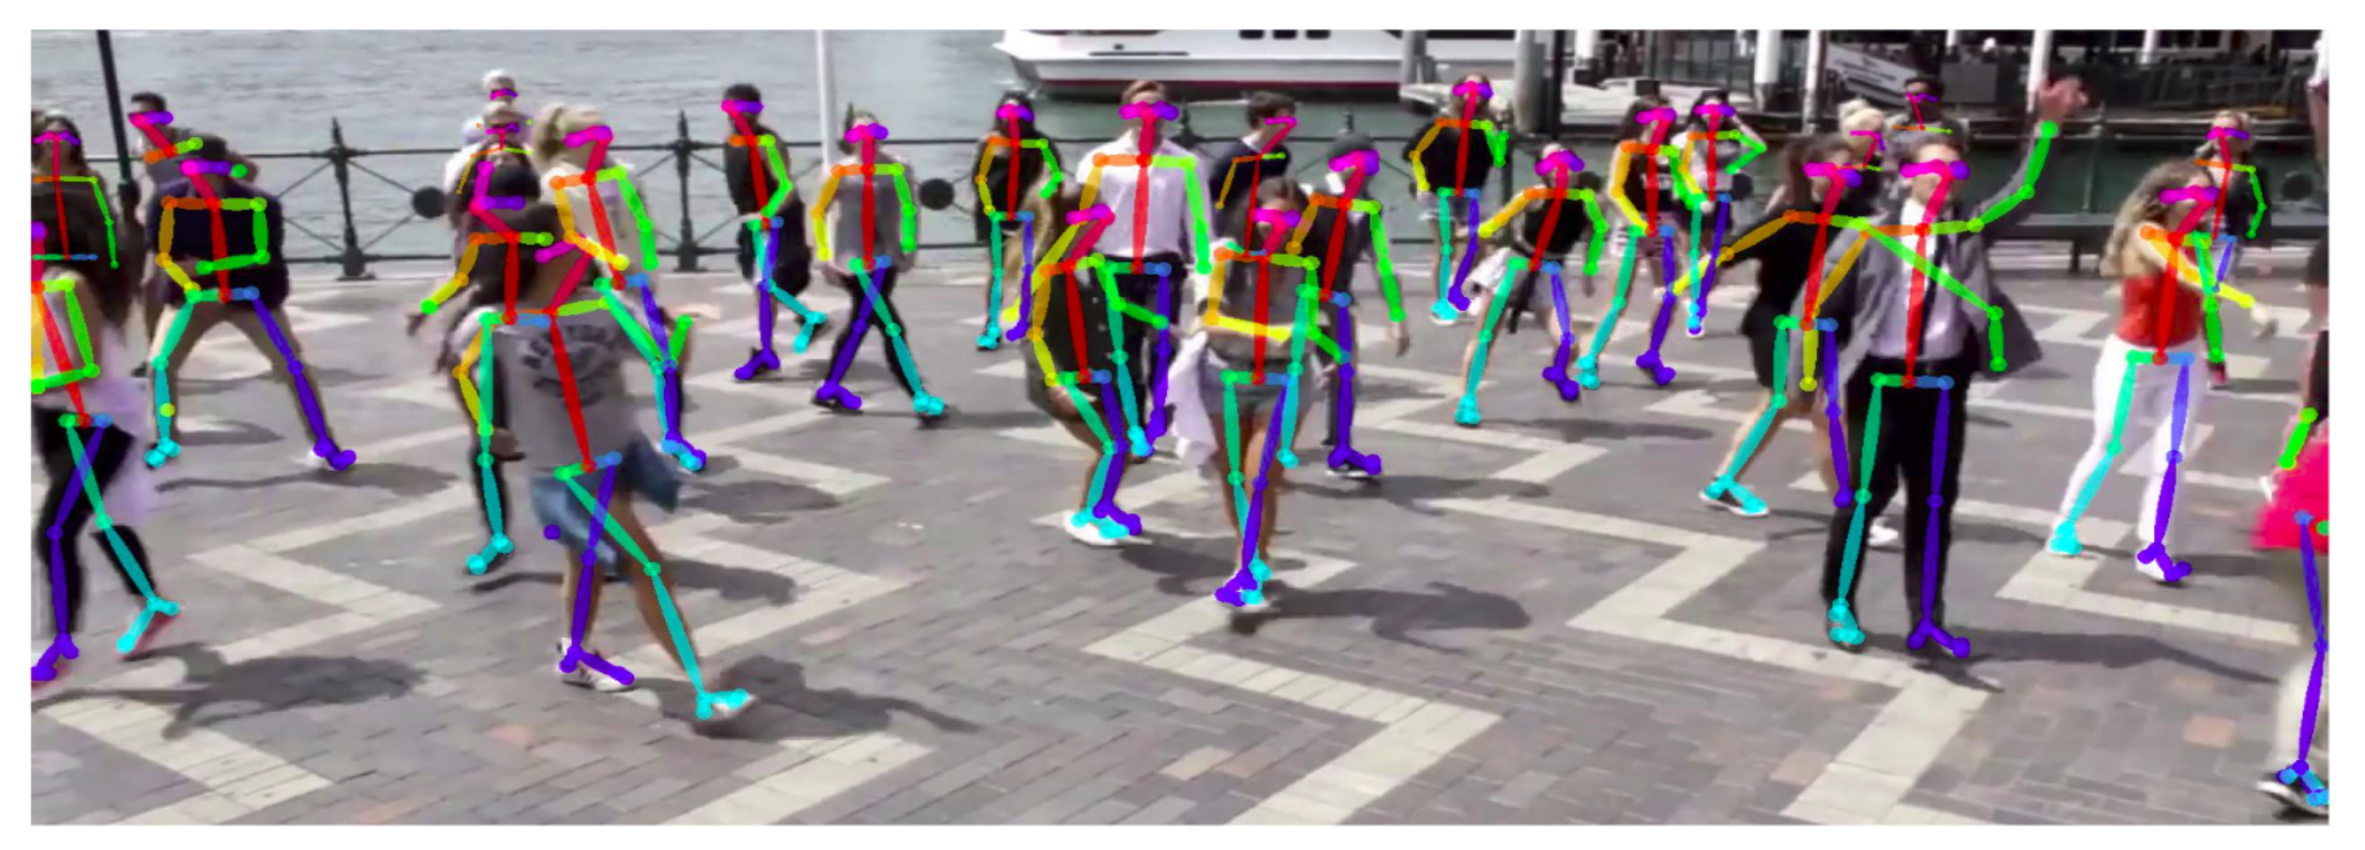
\includegraphics[width=\textwidth]{figures/openpose_demo.eps}
	\caption[Realtime multi-person 2D pose estimation using OpenPose algorithm]
	{Realtime multi-person 2D pose estimation using OpenPose algorithm that is independent of the number of people in the image. [Image courtesy Cao et al.~\cite{Cao_19}] \label{fig:openpose_demo}}
\end{figure}
\subsection{Techniques for Pose Estimation} 
There are two overarching approaches to pose estimation: a \textit{bottom-up} approach, and a \textit{top-down }approach.

With a bottom-up approach, the model detects every instance of a particular keypoint in a given image and then attempts to assemble groups of keypoints into skeletons for distinct objects. In simpler terms, the algorithm first predicts all body joints present in the image. This is typically followed by the formulation of a graph, based on the body model, which connects joints belonging to the same human. Integer linear programming (ILP) or bipartite matching are two common methods of creating this graph.

While, a top-down approach involves a segmentation step at the start. The network first uses an object detector to draw a box around each instance of an object and then estimates the keypoints within each cropped region. 

The potential simplest model for pose estimation used \gls{dnn}-based regressor to predict X, Y, and potentially Z coordinates for each keypoint location from an input image. In practice, however, this architecture does not produce accurate results without additional refinement. 

A slightly more complicated approach employs a deep learning-based encoder-decoder architecture. In this type of approach, instead of estimating the keypoint coordinates directly, the encoder is fed into a decoder, which creates heatmaps representing the likelihood that a keypoint is found in a given region of an image. During post-processing, the exact coordinates of a keypoint are found by selecting heatmap locations with the highest keypoint likelihood. In the case of multi-pose estimation, a heatmap may contain multiple areas of high keypoint likelihood (e.g. multiple right hands in an image). 

In top-down approach, an object detection module is placed between the encoder and decoder which is used to crop regions of an image likely to contain an object. Keypoint heatmaps are then predicted individually for each box. Rather than having a single heatmap containing the likely location of all of the specific body part in an image, we get a series of bounding boxes that should only contain a single keypoint of each type. 

So, top-down approach makes it easy to assign the keypoints to specific instances without a lot of post-processing. However, it suffers greatly when the person detector fails due to close proximity among people. Furthermore, their runtime is proportional to the number of people in the image. Contrarily, bottom-up approaches show robustness to early commitment and have the potential to decouple runtime complexity from the number of people in the image~\cite{Cao_19}.



\subsection{Introduction to OpenPose Library} 
\begin{figure}
	\centering
	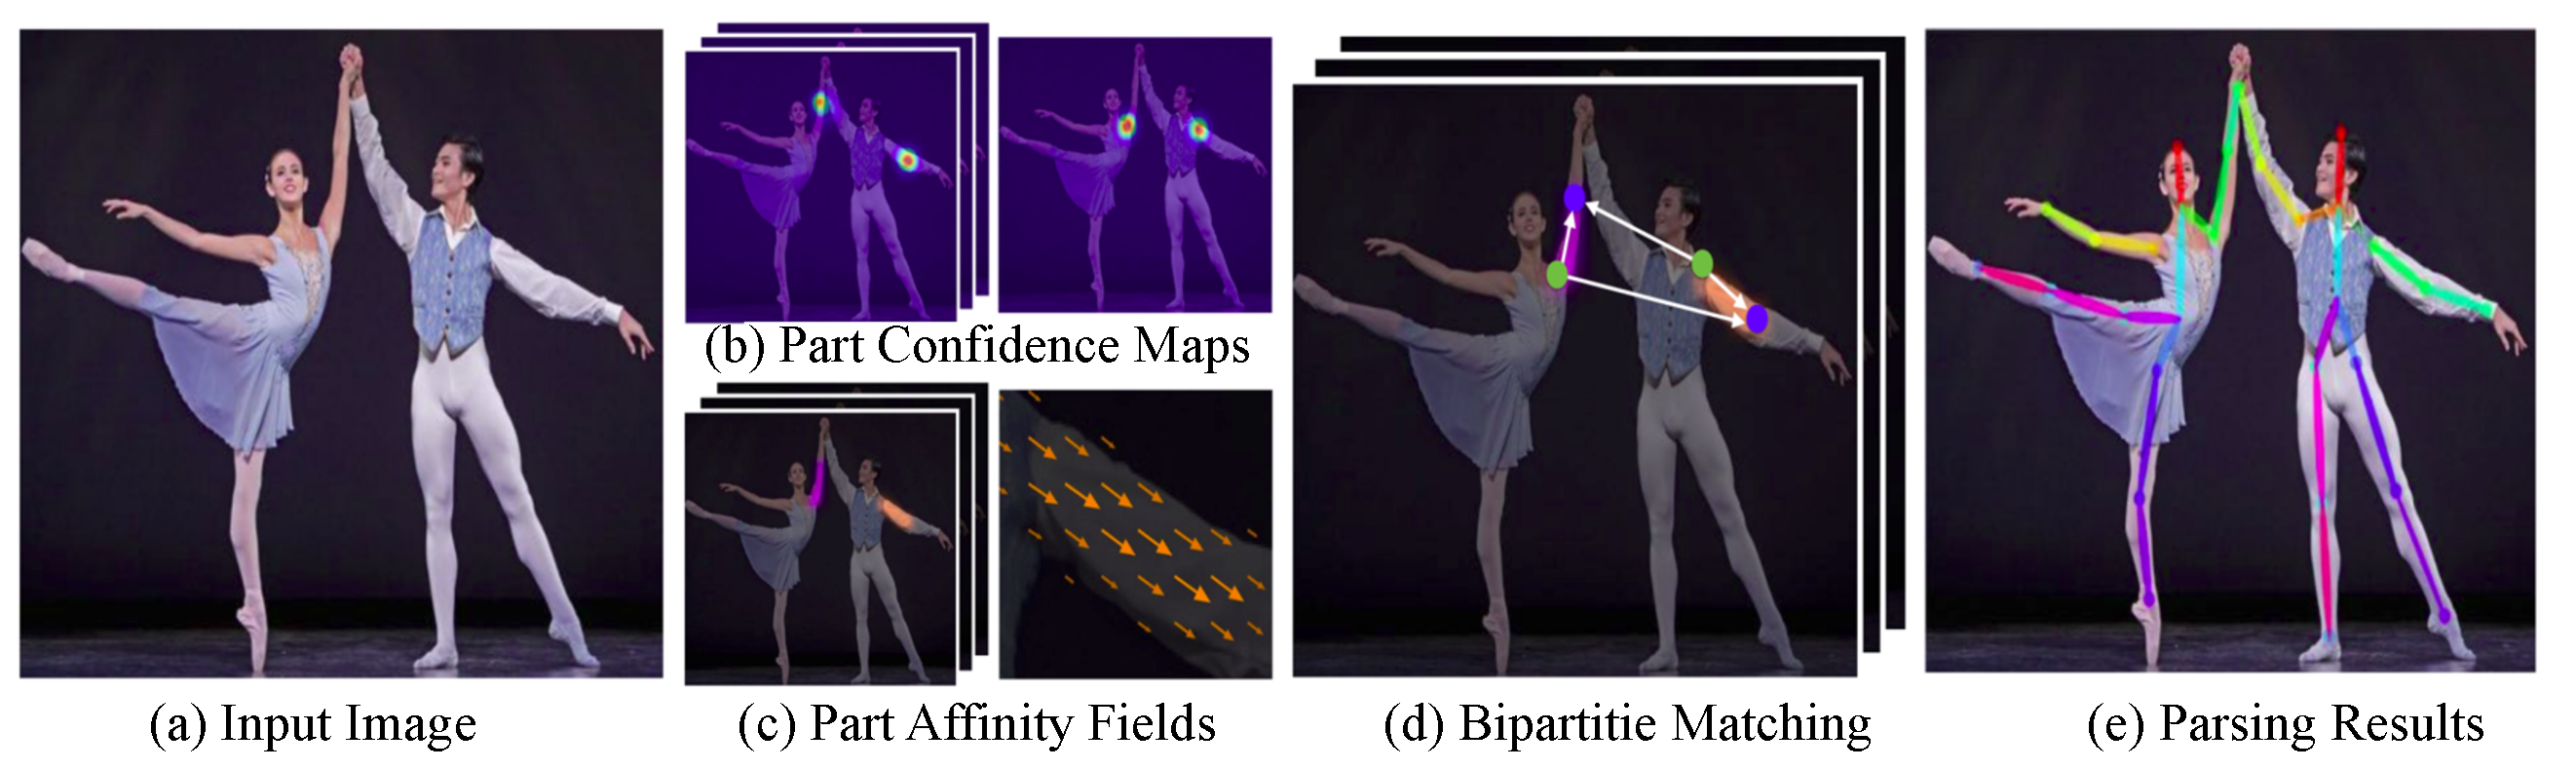
\includegraphics[width=\textwidth]{figures/openpose_bottom_up.eps}
	\caption[An example of a bottom up approach]
	{An example of a bottom up approach. [Image courtesy Cao et al.~\cite{Cao_19}] \label{fig:openpose_bottom_up}}
\end{figure}

\begin{figure}
	\centering
	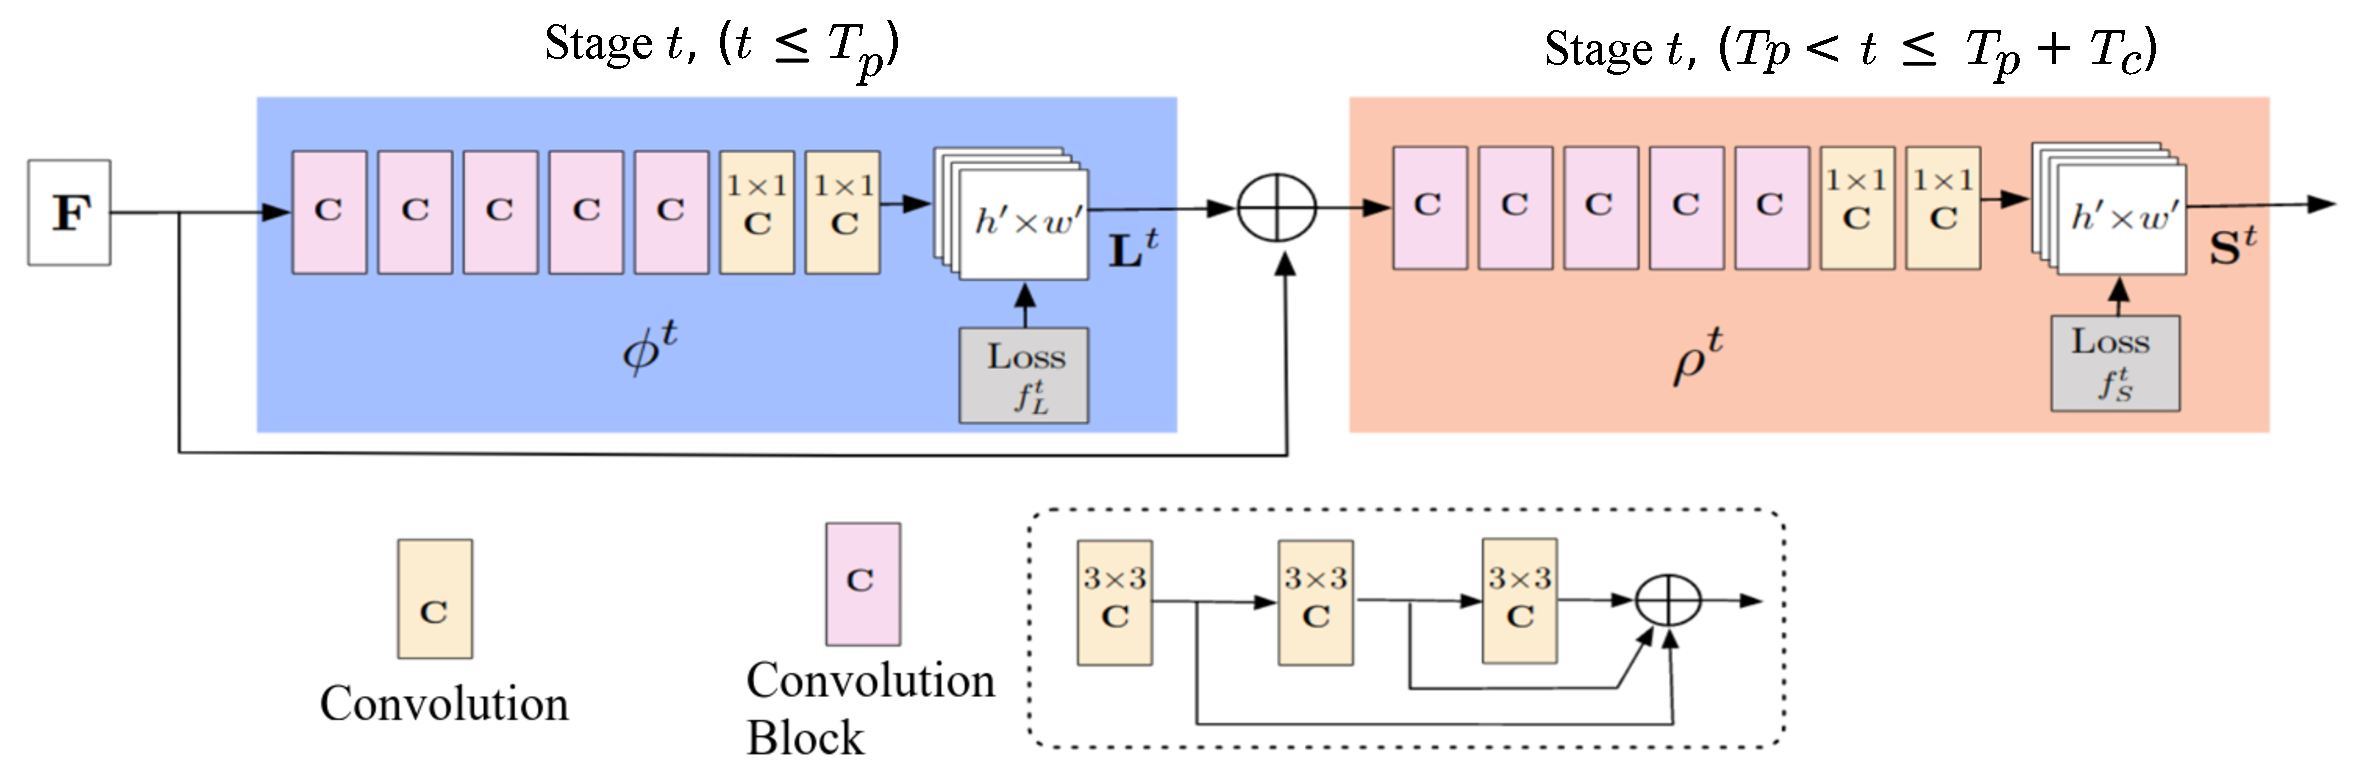
\includegraphics[width=\textwidth]{figures/openpose_architecture.eps}
	\caption[Network architecture of the multi-stage CNN]
	{Network architecture  of  the  multi-stage  CNN.  The  first  set of stages predicts PAFs $\textbf{L}^t$, while the last set predicts confidence  maps $ \textbf{S}^{t}$. [Image courtesy Cao et al.~\cite{Cao_19}] \label{fig:openpose_architecture}}
\end{figure}

In this research, we have employed OpenPose~\cite{Cao_19}, an open-source library for realtime multi-person 2D pose detection including body, foot, hand, and facial keypoints. This bottom-up approach achieves state-of-the-art accuracy in realtime performance. 

The overall pipeline of the OpenPose library is illustrated in Figure~\ref{fig:openpose_bottom_up}. An RGB image(Figure~\ref{fig:openpose_bottom_up}a) is fed as input to the library and it outputs the 2D locations of anatomical keypoints for each person in the image (Figure~\ref{fig:openpose_bottom_up}e). Firstly, a feedforward network predicts a set of 2D confidence maps \textbf{S} of body part locations (Figure ~\ref{fig:openpose_bottom_up}b) and a set of 2D vector fields \textbf{L} of part affinity fields (PAFs), which encode the degree of association between parts (Fig. ~\ref{fig:openpose_bottom_up}c). The set $\textbf{S} = (\textbf{S}_1,\textbf{S}_2,...,\textbf{S}_J)$ has $ J $ confidence maps, one per part, where $\textbf{S}_j \epsilon \mathbb {R}^{w\times h}$ . The set $\textbf{L}= (\textbf{L}_1,\textbf{L}_2,...,\textbf{L}_C)$ has C vector fields, one per limb, where $\textbf{L}_c \epsilon \mathbb {R}^{w\times h\times 2}$. Each image location in $\textbf{L}_c$ encodes a 2D vector. Finally, the confidence maps and the PAFs are parsed by greedy inference (Figure ~\ref{fig:openpose_bottom_up}d) to output the 2D keypoints for all people in the image. The network architecture of OpenPose algorithm, shown in Figure~\ref{fig:openpose_architecture}, iteratively predicts affinity fields that  encode part-to-part association.




\begin{figure}
	\centering
	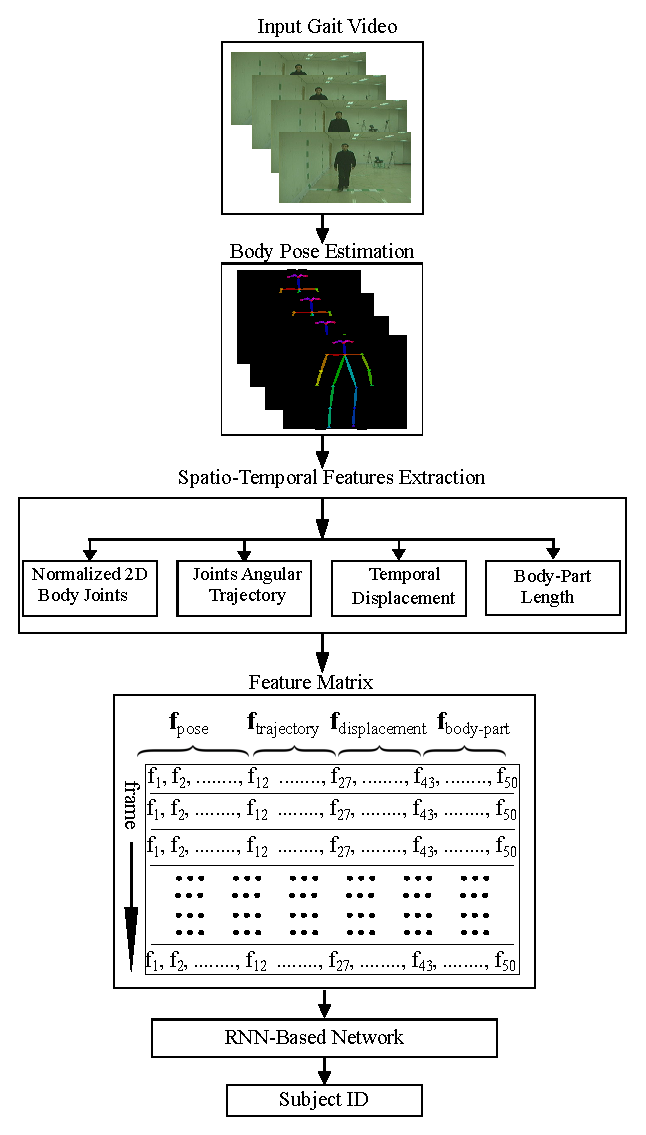
\includegraphics[width=0.8\textwidth]{figures/proposed_method.eps}
	\caption [The overview of the proposed framework for gait recognition] 
	{The overview of the proposed framework for gait recognition. 2D human poses were first extracted from raw video frames using improved OpenPose~\cite{Cao_19} algorithm. Four different types of spatio-temporal features were then extracted to form a 50-dimensional feature vector. Thereafter a pose sequence of timestep each having a length of 28 frame was formed to feed into a temporal network. The temporal network identified the subject by modeling the gait features. \label{fig:overview_proposed_method}
	}	
\end{figure}

%-------------------------------------------------------------------------
\section{Extracting Spatio-Temporal Feature Vector}
The workflow of the proposed network is illustrated in Figure~\ref{fig:overview_proposed_method}. Many strategies have been taken to designed a lower-dimensional spatio-temporal feature descriptor based on the 2D human poses estimated from the raw video frames. In this section, we elaborate the feature extraction procedure of our proposed method. 

\subsection{2D Body Joint Features}
As all the joints in the human body do not play a significant role in gait pattern, they cannot improve gait recognition accuracy. Some joints perform even worse. So, among the 25 body joints estimated from the OpenPose algorithm, we searched out for those joints which have a rich and discriminative gait representation capacity. Cunado \textit{et al.}~\cite{Cunado_97} used the human leg-based model as they found that change of human leg contains the most important features for gait recognition.  In our study, we found that knee along with the joints located in the feet show more robustness than any other body joints because they do not alter while people are walking in cloths or carrying bags. Some joints, e.g. hip, get wider in coat than normal condition. Again, in some gait videos, some subjects put their hands into their coat pocket, which they cannot do in normal walking. This situation significantly changes the joint coordinates. Therefore, raw body joints above hip do not have any significant impact on gait pattern. Hence, in our method, we did not consider hip or any other body joints above it.

\begin{figure}
	\centering 
	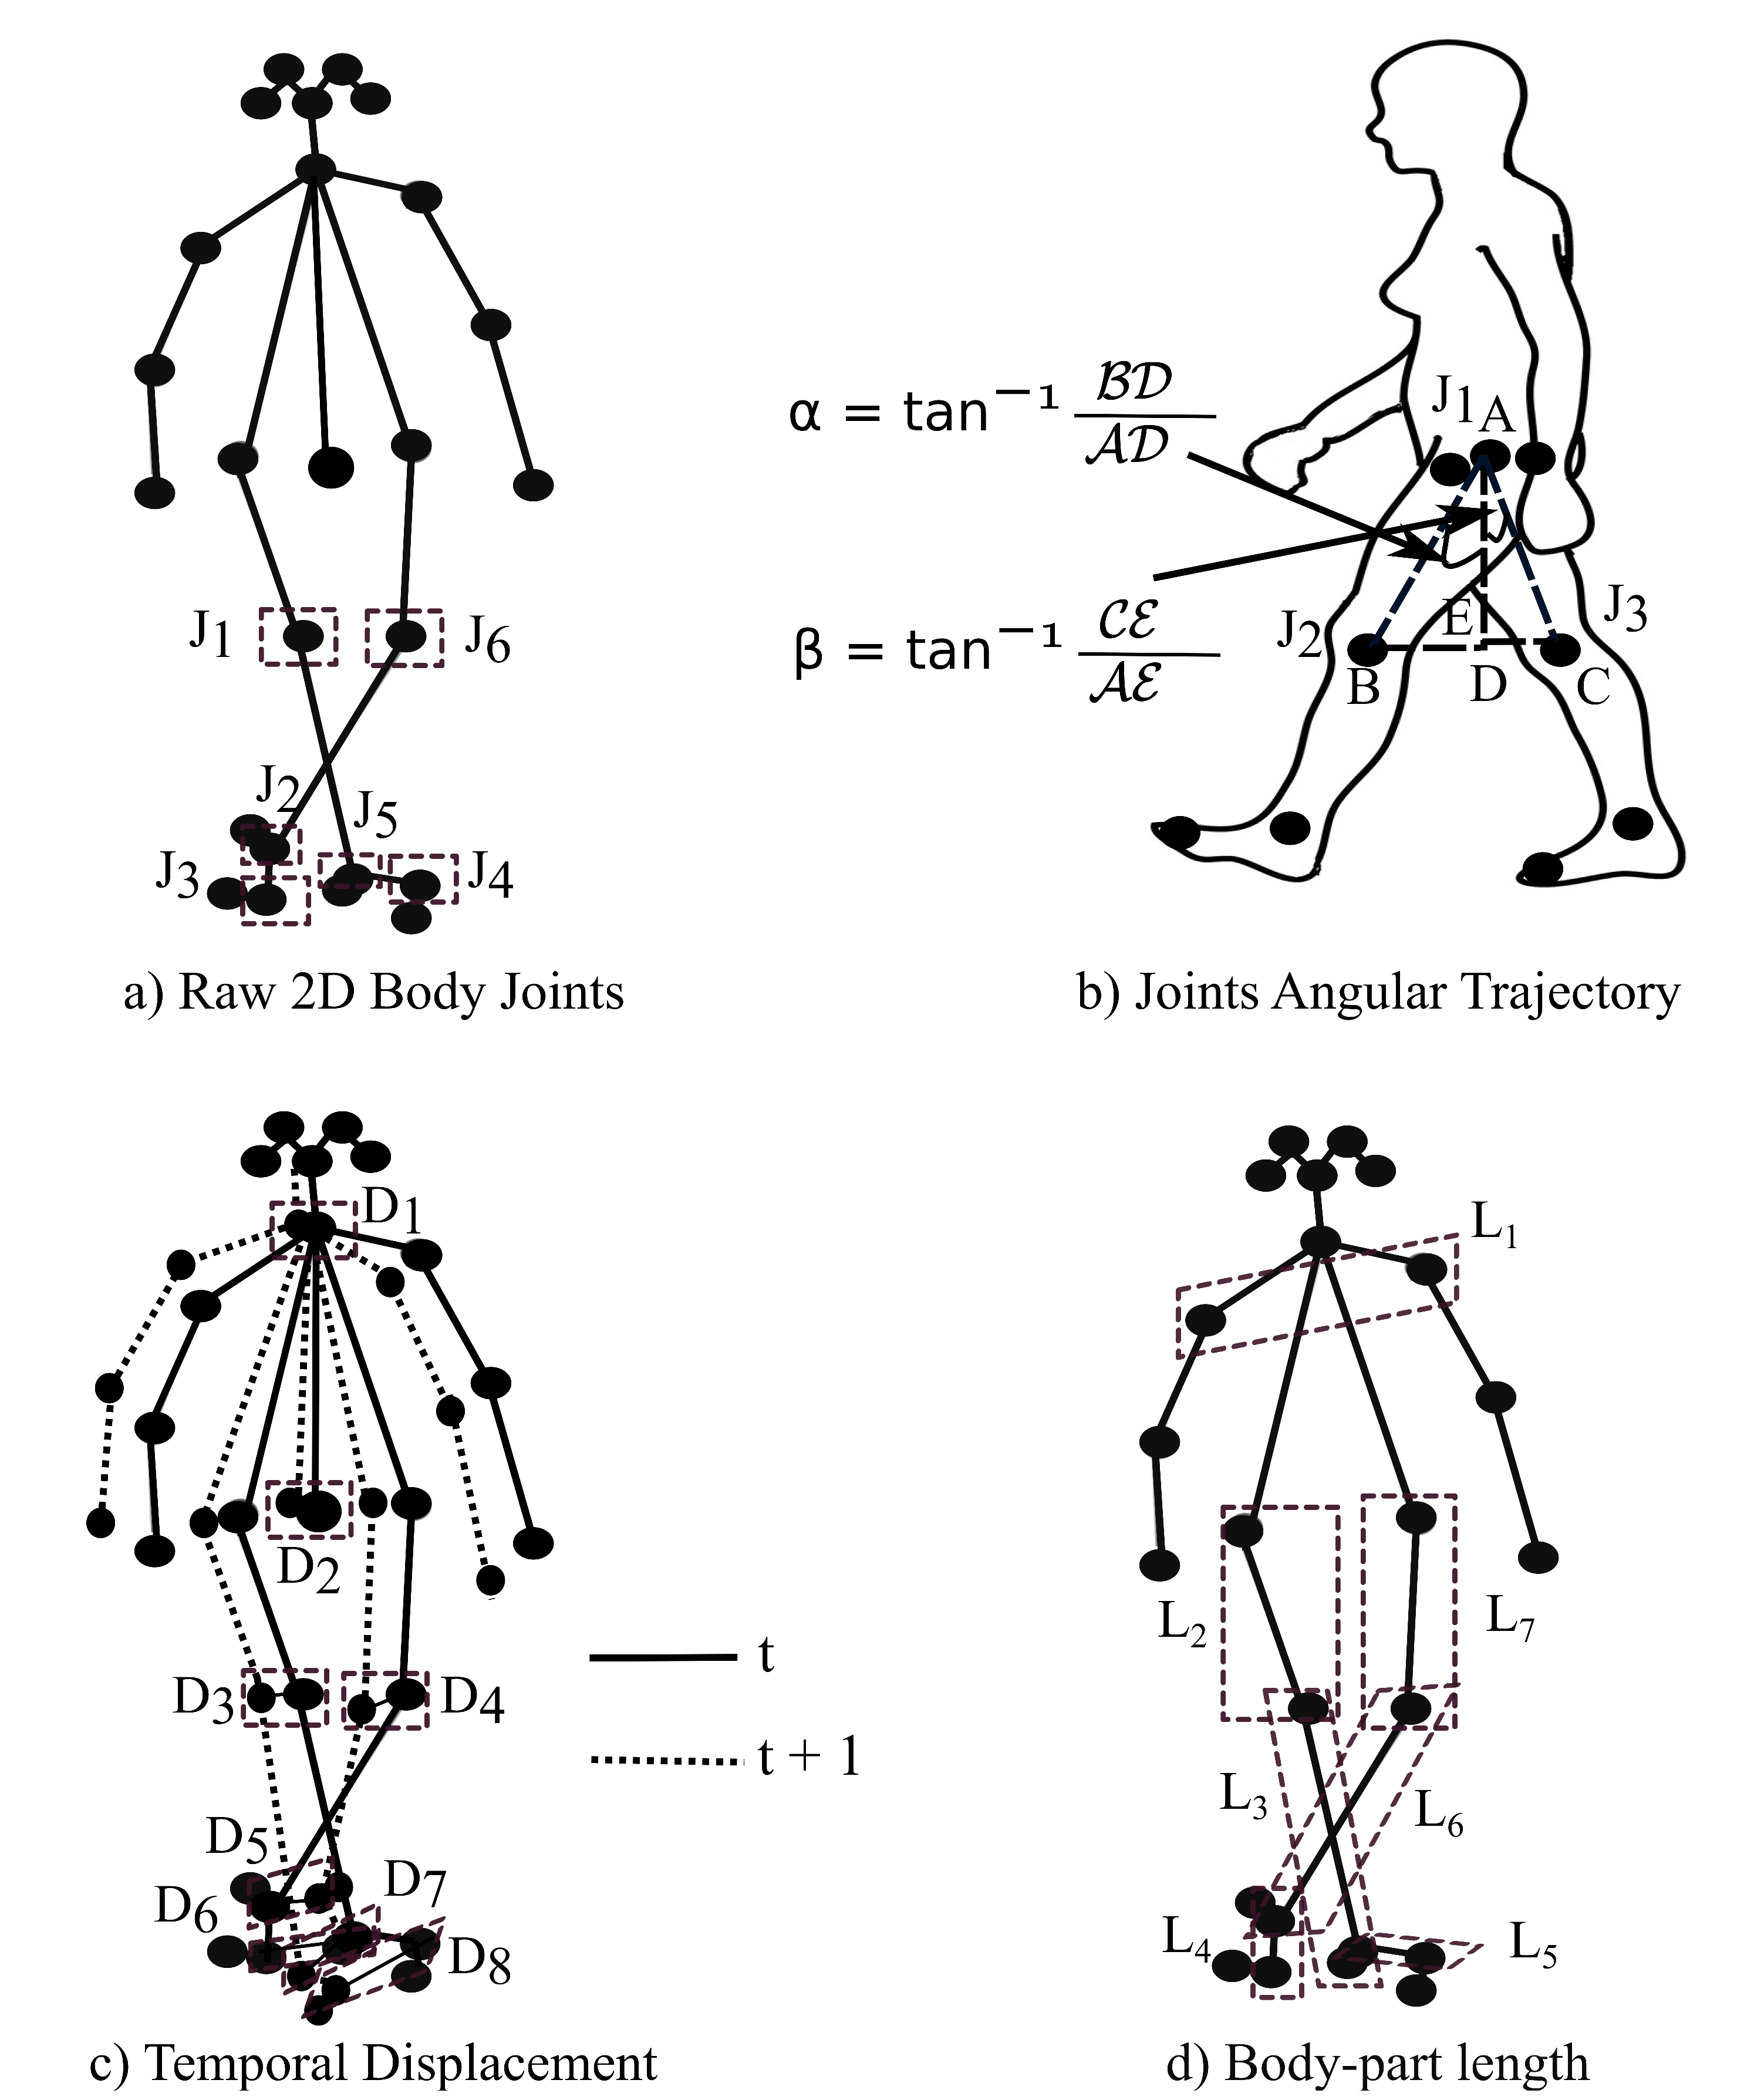
\includegraphics[width = 0.9\textwidth]{figures/extracted_features.eps}
	\caption[Scheme for the four different types of feature extraction process of the proposed method]
	{Scheme for the four different types of feature extraction process of the proposed method. a) 6 effective joints were selected out of 25 body joints. These selected joints formed a 12-dimensional pose vector. b) 5 angular trajectories from the lower limbs were considered to form a joint-angle feature vector. c) A total of 8 body joints were selected to get a temporal displacement feature vector. d) 7 body parts were taken to form a body part length feature vector.\label{fig:extracted_features}
	}
\end{figure}

Consequently, in our work, as shown in Figure~\ref{fig:extracted_features}a, we selected 6 body joints (RKnee, Rankle, RBigToe, LKnee, LAnkle, LBigToe) to form our effective body pose features. Thus, we have 12-dimensional pose feature vector, $\textbf{f}_{body-joint}$, for a single frame. 

\begin{equation}
  \textbf {f}_{body-joint}= [x_1, y_1, x_2, y_2, \ldots\ldots, x_6, y_6]^T
\end{equation}

It is necessary to normalize the pose sequence data with regard to the subject position in frame, size, or speed of walking to get improved performance. Now, in different gait datasets, as people walk through the fixed camera, the size of the subject's body alters due to variation in the distance between the subject and the camera. Therefore,  in order to eliminate different sizes and location variations of the human skeleton we had to transform the 2D  coordinates of all joints into a new coordinate system whose origin was selected as the middle of the hip ($\mathbf{J}_{o}$). To find the origin of the coordinate system ($\mathbf{J}_{o}$) for each subject, we considered the right, left, and middle of the hip joints and calculated the average of them. 

\begin{equation} 
\begin{split}
\mathbf{J}_{o} = {(x̄_{o} , y_{o})} &= {(\mathbf{J}_{LHip} +\mathbf{J}_{RHip} +\mathbf{J}_{MHip})} / {3} \\
(\bar{x}̄_{i} , \bar{y}_{i}) & = {(x̄_{i} , y_{i})} - {(x̄_{o} , y_{o})}~~~~\forall j \epsilon \mathbf{J}
\end{split}
\end{equation}
Here, $(\bar{x}̄_{j} , \bar{y}_{j})$ is set by root-centered coordinate reference system defined by above equations. Again, we normalized the skeletons of different subjects to fixed size by considering $ h $, the euclidean distance from hip to neck joint, as unit length. The following equation shows the normalization procedure of the raw 2D joints.


\begin{equation} \label{equ:normalization_raw_joint}
\begin{split}
	h &= \parallel \mathbf{J}_{o} - \mathbf{J}_{neck} \parallel_2  \\
	\mathbf{J}_{i}^{N} &= (\bar{\bar{x}̄}_{i} , \bar{\bar{y}}_{i}) = (\bar{x}̄_{i} , \bar{y}_{i}) / h 
\end{split}
\end{equation}
Here, $\mathbf{J}_{i}^N$ be the new coordinate of the $i^{th}$ joint $\mathbf{J}_{i}$ of a particular pose. These two steps of normalization have the huge impact on robustness of the gait recognition algorithm. Firstly, they allow fair comparisons between different subject's poses reducing the effect due to variation of subject size and position in the camera. Secondly, as it discards the absolute coordinates of subject's body pose, pose size become homogeneous among different camera settings and proximity to camera. Thus, it makes the system robust to zooming, camera position, and subject location. 



\subsection{Joint Angular Trajectory}
The dynamics of gait motion can be expressed by the temporal information of joint angles. Hence, discriminative gait features can be found by considering the change in joint-angle trajectories of the lower limbs~\cite{Wang_04}. Therefore, in this study, we formulated another 15-dimensional feature vector $\boldsymbol{f}_{trajectory}$ by considering five lower limb joint-angle trajectories using the following equations: 

\begin{table}
	\centering
	\caption{List of selected joint-angle trajectories with corresponding body joints set in order to form a joint angular feature vector. \label{table:list_joint_angle_trajectory}}
	\begin{tabular}{cc}
		\hline
		\textbf{Angular Trajectory} & \textbf{Body Joints Set}\\
		
		\hline
		Hip trajectory &10, 8, 13 \\
		Right knee trajectory  &11, 10, 9 \\
		Left knee trajectory &14, 13, 12 \\
		Right ankle trajectory &22, 11, 10 \\
		Left ankle trajectory &19, 14, 13 \\
		\hline
	\end{tabular}
\end{table}

\begin{equation}
	\begin{split}
	\alpha &= 
	\begin{cases}
	\tan^{-1}{\frac{|J_{2,x}-J_{1,x}|}{|J_{2,y}-J_{1,y}|}} & J_{2,y} \neq J_{1,y}\\
	\pi/2 & J_{2,y} = J_{1,y}
	\end{cases} \\ \noalign{\vskip10pt}
	\beta &= 
	\begin{cases}
	\tan^{-1}{\frac{|J_{3,x}-J_{1,x}|}{|J_{3,y}-J_{1,y}|}} & J_{3,y} \neq J_{1,y}\\
	\pi/2 & J_{3,y} = J_{1,y}
	\end{cases} \\ \noalign{\vskip10pt}
	\theta &= \alpha + \beta
	\end{split}
\end{equation}

As shown in Figure~\ref{fig:extracted_features}b, $J_1, J_2, J_3$ are the joints which form a set of angular trajectory. In this work, we considered total five sets of angular trajectories from the lower limb of human body. Table~\ref{table:list_joint_angle_trajectory} demonstrated the selected angular trajectories with their corresponding body joints. For each trajectory, we took $(\theta, \alpha, \beta)$ as gait features. 

\begin{equation}
\textbf {f}_{trajectory}= [\theta_1, \alpha_1, \beta_1,\theta_2, \alpha_2, \beta_2,\ldots\ldots, \theta_5, \alpha_5, \beta_5]^T
\end{equation}


\subsection{Temporal Displacement}
Our third type of feature extractor is a simple descriptor that preserves temporal information of the gait pattern. It basically stores the local motion features of gait by keeping the displacement information between the two adjacent frames of the subject's pose sequence. The displacement of each coordinate of a joint was then normalized by the total length of displacement of all joints. Let, $t$ and $(t + 1)$ are two adjacent frames of a particular pose sequence. Now, the displacement information of the coordinates of any joint of frame $t$ would be the normalized difference between the corresponding coordinates of two adjacent frames. 

\begin{equation}
\begin{split}
\triangle x^{t}_{1} &=\frac{x^{t+1}_{1} - x^{t}_{1}}{\sum_{i=1}^{8}\parallel J^{t+1}_{i,x} - J^{t}_{i,x}\parallel_2} \\ 
\triangle y^{t}_{1} &=\frac{y^{t+1}_{1} - y^{t}_{1}}{\sum_{i=1}^{8}\parallel J^{t+1}_{i,y} - J^{t}_{i,y}\parallel_2} \\ 
{\bf f}_{displacement} &= [\triangle x_{1}, \triangle y_{1}, \triangle x_{2}, \triangle y_{2} \ldots\ldots, \triangle x_{8}, \triangle y_{8}]^{T}
\end{split}
\end{equation}

Here, $J_i^{t}$ is the 2D coordinates of the $i_{th}$ body joint at $t^{th}$ frame in the video and $(\triangle x_1^t , \triangle y_1^t )$ is the displacement of the coordinates of first joint at $t^{th}$ frame of the video. As shown in Figure~\ref{fig:extracted_features}c, we selected 8 joints (Neck, MHip, RKnee, Rankle, RBigToe, LKnee, LAnkle, LBigToe) to get a 16-dimensional feature vector, $\textbf{f}_{displacement}$.


\subsection{Body Part Length Features}
The static gait parameters, for example, the length of the body parts calculated from raw body joints position are also very important for gait recognition~\cite{Wang_04, Araujo_13}. They form a spatial gait feature vectors which make them robust against covariate factors such as carrying and clothing condition variation. In this study, we took seven body parts (Figure~\ref{fig:extracted_features} (d)) namely length of the two leg, two feet, two thigh and width of the shoulder which formed a 7-dimensional spatial feature vector $\textbf{f}_{body-part}$. 


\subsection{Fusion of Features}
A lot of research works have been done to fuse multiple features to get improved performance~\cite{Liao_19, Wang_04}.  Different types of fusion methods were proposed in literature such as feature level fusion, representation level fusion, and score level fusion. In feature level fusion, multiple features of the same frame are concatenated before feeding into a final network and in representation level fusion, each feature vector is firstly fed into a network and the resulting global representations are then concatenated to train a final classifier. For score level fusion, each feature vector is separately fed into the final network which predicts a classification score. Then, the scores from multiple classifiers are fused using an arithmetic mean.

In this study, we found that feature level fusion has produced better recognition results in contrast to other fusion techniques or individual feature sets. 


\begin{figure}
	\centering 
	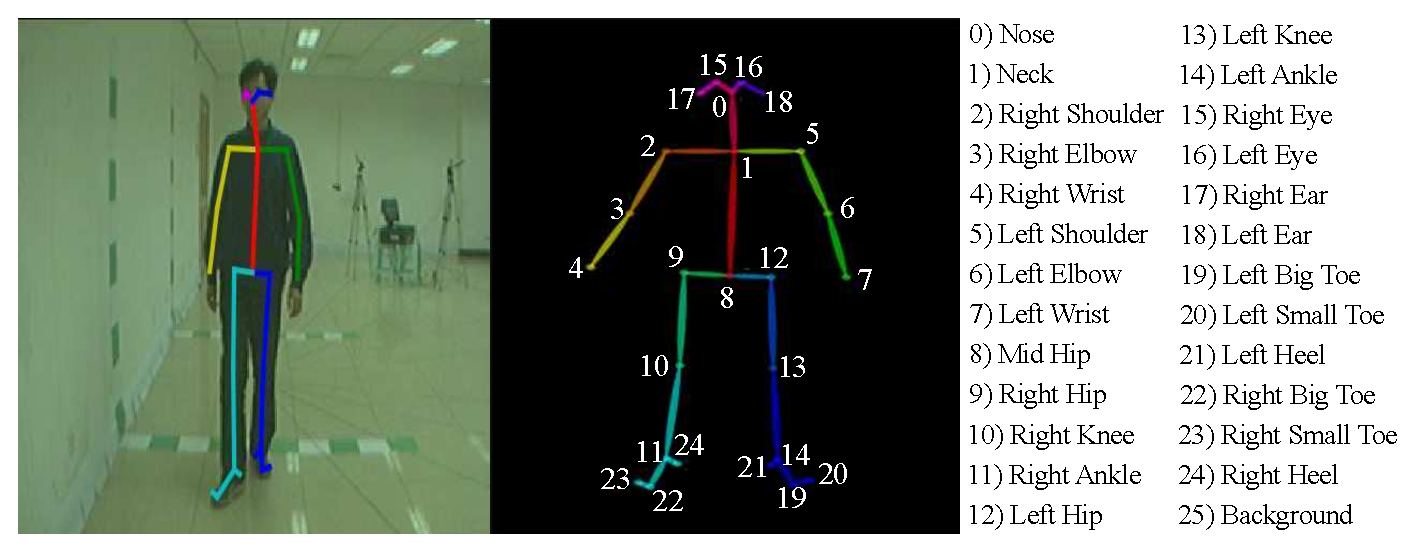
\includegraphics[width = \textwidth]{figures/pose_estimation.eps}
	\caption[Examples of 2D human pose estimation from RGB images of CASIA dataset]
	{Examples of 2D human pose estimation by~\cite{Cao_19} from RGB images of CASIA dataset (left ones). Detected 25 human body joints with description are shown. (right ones) \label{fig:pose_estimation}
	}
\end{figure}



%-------------------------------------------------------------------------
\section{Feature Preprocessing}
From 2D pose estimation algorithm~\cite{Cao_19}, we got raw 2D coordinates for each joint, as shown in Figure~\ref{fig:pose_estimation}. In this work, several preprocessing steps have been undertaken to build a compact, robust and discriminative descriptor based on these raw coordinates. In this section, we are going to discuss these steps in detail.



\subsection{Handling Missing Joint Information}
One of the most challenging tasks for pose estimation algorithm to estimate the pose of a subject who is completely or partially occluded. This scenario often leads the algorithm to fail in estimating one or more joint coordinates. In order to make our proposed gait algorithm robust and accurate, we have to address the problem of missing joint information carefully. The main strategies we have taken in this work are: 

\begin{itemize}
\item If the origin of the coordinate system can't be calculated due to missing hip joints, the frame should be rejected;
\item If more than 1 body joint is missing in between knee and ankle joints of both leg, the frame should be rejected due to having little information;
\item Persistent missing joints can be guessed by exploiting the left and right side body symmetry;
\item In other cases, individual joints were not located in the frame and a position of $[0.0, 0.0]$ was given to that joint. 
\end{itemize}

The above strategies are simpler which do not require any computation and proven to be effective in addressing the missing data problem. Algorithm~\ref{alg:missing_data} depicts the proposed techniques for handling missing joint information.

\begin{algorithm}
	\caption{Algorithm for Handling Missing Joints Information}
	\label{alg:missing_data}
	\begin{algorithmic}
		\input{algorithms/missing_data.alg}
	\end{algorithmic}
\end{algorithm}

\subsection{Forming Feature Map}
In this thesis, we designed a 50-dimensional spatio-temporal gait feature vector \textbf{p} from the raw 2D pose estimation of each frame.  Firstly, we split a gait video into 28 frame segments. Each $28$ frame-segment formed a timestep which can be described by the following equations. 

\begin{equation}
\label{equ:feature_preprocess}
\begin{split}
\boldsymbol{p} &= {[f_1, f_2, f_3, \ldots \ldots, f_{50}]}^T \\
\boldsymbol {T} &= {[\boldsymbol p_1, \boldsymbol p_2, \boldsymbol p_3,  \ldots \ldots, \boldsymbol p_{28}]}^T \epsilon \quad \mathbb {R}^{28\times 50}\\
\boldsymbol V &= {[\boldsymbol T_1, \boldsymbol T_2, \boldsymbol T_3,  \ldots \ldots \boldsymbol T_{N}]}^T 
\end{split}
\end{equation}

Here, \textbf{p} is the 50-dimension pose vector for each frame; \textit{\textbf{T}} is the feature matrix for each timestep; $ N $ is the total number of timestep sequence, and \textit{\textbf{V}} is the sequence of features for a gait video. 



\subsection{Data Augmentation}
The performance of deep neural networks is strongly correlated with the amount of available training data. Although, CASIA~\cite{Yu_06} is the largest gait dataset, the standard experimental setup of this dataset (see Table ~\ref{table:caisab_setup}) allows us to train only the four normal walking sequence for each subject. Therefore, we need to augment our train data to obtain a stable model. One way to increase the amount of training data is to overlap video clip. So, we split the input video into an overlapping sequences of video clips. For every 28 image clip, we overlapped 24 images of the previous clip at almost $ \textbf{85.7\%} $ overlapping rate. For example, a particular gait video of 100 frames would be split into the clips $(1-28), (5-32), (9-36), ...$ up to frames $(73, 100)$. 

Again, in CASIA dataset, gait videos of different subject have varying timesteps. The number of timesteps in each gait video depends on the total number of frames where a person is detected. Due to the position of the camera, some angles ${(0^{\circ}, 18^{\circ}, 36^{\circ})}$ have more person detected frame than other angles ${(72^{\circ}, 90^{\circ}, 108^{\circ})}$. Therefore, the total number of timesteps in a gait video is different for different subjects and view angles. This varying timestep makes our train dataset unbalanced. Again, in CASIA B dataset, every subjects have not have all gait videos; there are some missing gait videos. To solve the problem, for improved performance we have to develop our own balance training set by making each subject pose sequence to have a fixed number timesteps. We first found the subject which had maximum timesteps for a particular gait angle and then augmented other subject's timesteps with that specific length by overlapping their sequences.

In addition to above technique, we further augment our training data by adding another gait sequence (i.e., $ 25\% $ increment) by implementing Gaussian noise to a given normal walking sequence. 

\begin{equation}
N(j_i) = (x + \tilde{x},  \quad y+ \tilde{y})
\end{equation}

Here,  $\tilde{x}$ and $\tilde{y}$ are two random real numbers generated by a normal distribution with zero mean and unit standard deviation. We apply noising ($ N $) into the raw joints position of a training pose data.



%-------------------------------------------------------------------------
\section{Single-View Gait Recognition}
In this section, we will present the details of the architecture and training procedure of our proposed network for single-view gait recognition. We will also try to describe why our proposed 2-layer BiGRU network is best in modeling the gait descriptors for recognizing the subject ID.

\subsection{Network Architecture}
\begin{figure}
	\centering 
	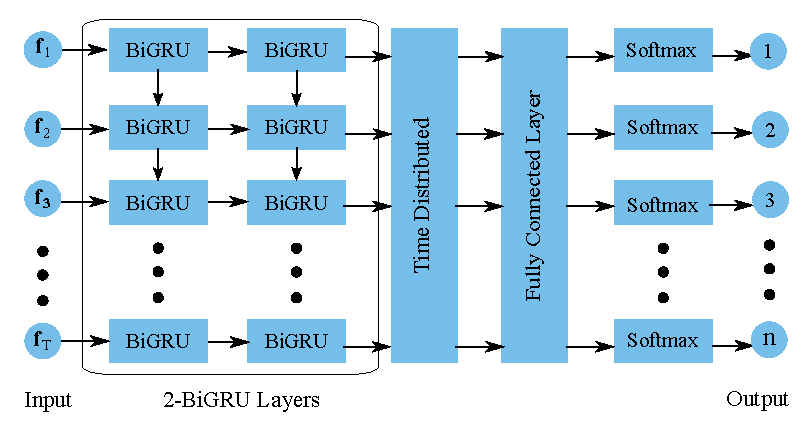
\includegraphics[width = \textwidth]{figures/rnn_network.eps}
	
	\caption[Proposed network architecture for robust gait recognition]
	{Proposed network architecture for robust gait recognition. It consists of two \gls{bigru}~\cite{Schuster_97} layers each of which consists of $ 80 $ \gls{gru} cells with one batch normalization. The network was fed with a 50-dimensional spatio-temporal feature vector obtained from 2D pose estimation. Input layer was followed by a batch normalization layer~\cite{Ioffe_15}. The output of the recurrent layers was also batch normalized to standardize the activations and finally fed into an output softmax layer. For the output layer, the number of the output neuron equals to the number of subjects. \label{fig:rnn_network}
    }
\end{figure}


In this research, we experimented with different \gls{rnn} architectures such as gated recurrent units (\gls{gru}s),  long short-term memory units (\gls{lstm}s), bidirectional long short-term memory (\gls{bilstm})~\cite{Graves_05} and bidirectional gated recurrent units (\gls{bigru})~\cite{Schuster_97}. Firstly, we designed the proposed network employing all these architectures with one recurrent layer and then, searched for optimum recurrent unit size between 50 to 150. Thereafter, we increased the capacity of the network by adding the second and third layers of hidden units. Finally, we found that, among different RNN architectures, 2-layer \gls{bigru} with 80 hidden units performs best. Therefore, we chose \gls{gru} in our proposed network architecture as it achieves high performance and requires a reduced number of parameters while still retaining long-term temporal information.

After input and the second recurrent layer, we placed a batch normalization (\gls{bn})~\cite{Ioffe_15} layer. At last, a fully connected layer with softmax activation was used to predict the subject classes. Figure~\ref{fig:rnn_network} illustrates the architecture of the proposed network. 


\subsection{Loss Function}
In this work, we found that due to the influence of various covariate factors, intraclass distance related to one subject is sometime more significant than interclass distance. So, if we only use the \textit{cross-entropy loss} as our objective function, the resulting learned features may contain large intraclass variations. Therefore, to effectively reduce the intraclass variations, we employed \textit{center loss} as introduced by Wen \textit{et al.}~\cite{Wen_16} for face recognition task. 

Now, as the training progresses, the center loss learns a center for the features of each class. Also, the distances between the features and their corresponding class centers are minimized simultaneously. However, using only center loss may lead the learned features and the centers close to zeros due to the very small value of the center loss. Hence, with the fusion of softmax loss ($L_s$) and center loss ($L_c$), we can achieve discriminative feature learning by increasing interclass dispersion and compacting intraclass distance as much as possible.


\begin{equation} \label{equ:loss_functions}
\begin{split}
L_s &=-\sum_{i=1}^{m}log{\frac{e^{W_{y_i}^{T}x_i + b_{y_i}}}{\sum_{j=1}^{n}{e^{W_{j}^{T}x_i+ b_j}}}} \\
L_c &= \frac{1}{2}\sum_{i=1}^{m}{\parallel{{\boldsymbol x_i}-{\boldsymbol c_{y_i}}}\parallel}_2^2 \\
L &= L_s + \lambda L_c + \lambda_{\theta}\parallel{\theta}\parallel_{2}
\end{split} 
\end{equation}

Equations~(\ref{equ:loss_functions}) describe the total loss ($ L $) calculation of our proposed network. where $\boldsymbol x_{i} \epsilon \mathbb {R}^d$ denotes the $i^{th}$ pose sequence which belongs to the $y_i^{th}$ class and  $\boldsymbol c_{y_i} \epsilon \mathbb {R}^d$ denotes to the $y_i^{th}$ class center of the learned pose features. $W \epsilon \mathbb {R}^{d\times n}$ is the feature dimension of the last fully connected layer and $b\epsilon \mathbb {R}$ is the bias term of the network. The batch size and the class number are $ m $ and $ n $ respectively. $\lambda$, a scalar variable, is set to value $ 0.01 $ to balance between the two loss functions. $\parallel{\theta}\parallel_{2}$ refers to the kernel regularizer for all the parameters of the network with a weight decay coefficient $(\lambda_{\theta})$ set to $0.0005$ for the experiment.  


\subsection{Post-processing}\label{subsec_post_process}
While training, our proposed temporal network considered each of these video clips as a separate video (see Figure~\ref{fig:output_prediction}). For a given video, the prediction of our model is a sequence of class probabilities for each timestep, i.e. 28-frame clip.

\begin{figure}
	\centering
	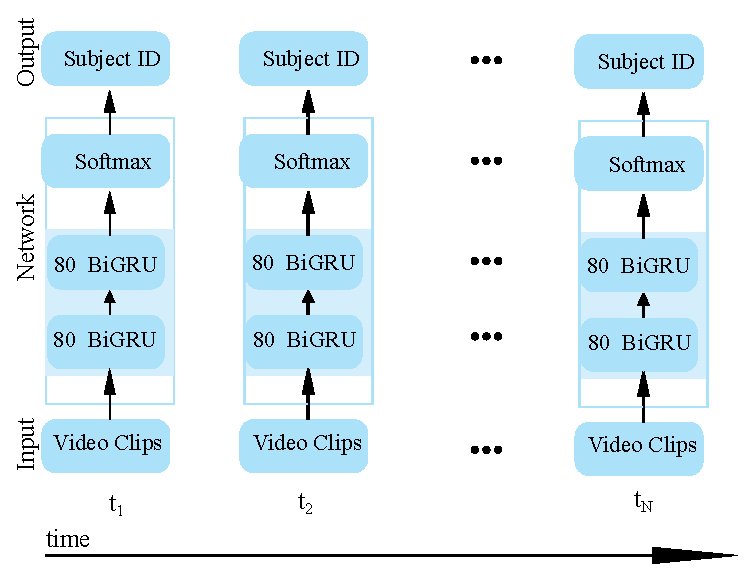
\includegraphics[width=0.7\textwidth ]{figures/output_prediction.eps}
	\caption[Output prediction scheme of our proposed network]{
		Output prediction scheme of our proposed network. Each input clip, a timestep of 28 frame, was considered as a separate video and a sequence of class probabilities was predicted at the output. Majority voting scheme was used to process the output to predict the subject ID.
	}
	\label{fig:output_prediction}
\end{figure}

But, while testing, we actually need the subject ID for the complete gait video. Therefore, we used \textit {majority voting scheme} to process this output to predict the subject ID. In this scheme, the subject that receives the highest number of votes over all timesteps in a  gait video is referred as the predicted class.

Let's consider, $\boldsymbol{s}$ is a vector IDs for $n$ number of subjects. For a particular timestep $t$, a gait video has input feature map $\boldsymbol X^t \epsilon \mathbb {R}^{28\times 50}$ and an n-dimensional output vector $\boldsymbol o^t$.

\begin{equation} \label{equ:timestep_sequence}
\begin{split}
\boldsymbol s^t &=  {[s_1, s_2, s_3, ....., s_{n}]}^{T}\\
\boldsymbol o^t &=  {[o_1, o_2, o_3, ....., o_{n}]}^{T}
\end{split}
\end{equation}

Here, $o_i^t = P(s_i | X^t)$ refers the probability of input feature map $\boldsymbol X^t$ belongs to class $s_i$. Now, we assign the output class $\mathbf{o}^t$ to the subject class $s_i$ which have maximum probabilities for the timestep $t$. As each of our gait videos is divided into a series of timestep sequence (see equation~\ref{equ:timestep_sequence}), using majority voting scheme we can have the subject ID. Following equations described the voting scheme:

\begin{equation}
\label{equ:predicted_class}
\begin{split}
s_t &=  \arg\max_{s_i}{\{o_i^t | 1 \leq i \leq n\}} \\
s &= {\arg\max}_{i\in(1, 2, ...,n)}{\sum_{t=1}^{N}s_i^N}
\end{split}
\end{equation}

Here, $ N $ is the total number of timesteps in which a gait is split and $ s $ is the final predicted class.  


\subsection{Training and Implementation Details}
The training of \gls{rnn}s allows us to learn the parameters from the sequence. We have employed Adam~\cite{Kingma_15} optimization algorithm with $\beta_1 = 0.9$ and $\beta_2 = 0.999$, which is known to work very well for training \gls{rnn}s. We tried several learning rates in our experiment and found out that the best initial learning rate is $(5$x$10^{-3})$. We also reduced the learning rate by a factor when it hit a plateau. Reducing the learning rate will allow the optimizer to get rid of the plateaus in the loss surface. Table~\ref{table:summary_tn} summarizes all the hyperparameters setting of our network.

\begin{table}
	\centering
	\caption{Training summary of our proposed temporal network. \label{table:summary_tn}}
	\begin{tabular*}{32pc}{@{\extracolsep{\fill}}ll@{}}
		\hline \noalign{\vspace{3pt}}
		\textbf{Hyperparameter} &\qquad \textbf{Value} \\ [3pt] \hline\noalign{\vspace{3pt}}
		Optimizer     			&\qquad Adam~\cite{Kingma_15} \\[3pt]
		Objective function  	&\qquad Fusion of softmax and center loss \\[3pt]
		Epochs        			&\qquad $ 450 $ \\ [3pt]
		Initial learning rate	&\qquad $5 \times 10^{-3}$  \\[3pt]
		Mini-batch size			&\qquad $ 256 $ \\
		\hline
	\end{tabular*}
\end{table}

The proposed network was trained with a batch size of $ 256 $ for $ 450 $ epochs. Our network showed some overfitting mostly due to the high learning capacity of the network over data. We addressed the overfitting problem by adding a \gls{bn} layer before and after the \gls{bigru} layer. We also tried to add dropout layer during training, but that did not help to reduce the overfitting problem. Moreover, it degraded gait recognition performance. Hence, we skip it.

For the model computations, we entirely relied on GPU programming. In particular, our implementation was based on Keras~\cite{keras}, a GPU-capable deep-learning library written in Python. All the experiments were performed on a server machine with 56 cores, 512 GB RAM and a Nvidia Tesla K40 graphic card with 12 GB memory running on Ubuntu server 18.04 LTS. Input video and image sequences were processed using Python and OpenCV library~\cite{opencv}.




\begin{figure}
	\centering
	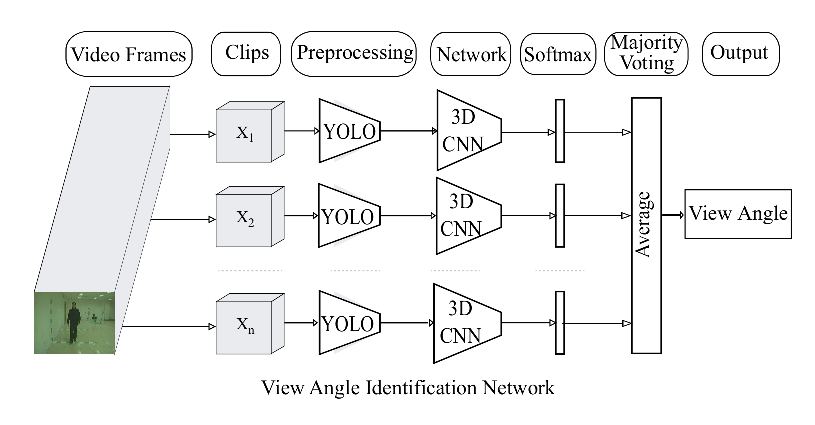
\includegraphics[width=0.9\textwidth]{figures/view_angle_identification.eps}
	\caption[Overview of our proposed view angle identification network scheme] 
	{Overview of our proposed view angle identification network scheme. YOLOv3~\cite{Redmon_18} was used to detect and locate the walking people in video frames. The input of the network was a clip of 16 consecutive frame which was preprocessed and resized to $112\times112$ to feed into a 3D convolutional network based on C3D~\cite{Tran_15}. The network used 3D kernels to exploit spatio-temporal dynamics for view angle identification. \label{fig:view_angle_identification}
	}
\end{figure}

%-------------------------------------------------------------------------
\section{Multi-View Gait Recognition}
In this section we will elaborate our propose two-stage network architecture for multi-view gait recognition. Here, in first stage, we trained a 3D convolutional network to estimate the walking direction of the subject by extracting spatio-temporal features from gait video. Thereafter, we performed subject identification using proposed temporal network which has been trained for that view angle.


\subsection{Preprocessing}
Firstly, to localize human walking in gait videos, we used YOLOv3, a state-of-the-art realtime object detection algorithm, proposed by Redmon \textit{et al.}~\cite{Redmon_18}. We then cropped each of the person detected frame using the bounding box coordinates found from YOLOv3 algorithm and resized them to $112\times112$ for our network input. Thereafter, we splitted each gait video into overlapping sequences of 16 consecutive frames within training or test set. There is an overlap of 8 frames (50\%) indicating that the samples were gathered using a 16 frame sliding window with a 50\% stride.


\subsection{3D Convolution for Video Classification}
Identifying walking direction from gait video is somewhat similar to action recognition problem in computer vision. Recently, in action recognition, researcher have started to exploit 3D features in video using 3D-CNN model which extracts features from both spatial and temporal dimensions by performing 3D convolutions. Tran et.al.~\cite{Tran_15} proposed a 3D convolutional neural network, also known as C3D, which has been widely used for applications like video classification, action recognition, etc. Sports-1M~\cite{karpathy_14}, one of the largest benchmark datasets for video classification has been employed to train the network. The dataset contains $ 1.1$ million sports videos, where each video belongs to one of the 487 sports categories. 


\begin{table}
	\centering
	\caption{Training summary of our proposed 3D-CNN network.  \label{table:summary_3dcnn}}
	\begin{tabular*}{30pc}{@{\extracolsep{\fill}}ll@{}}
			\hline \noalign{\vspace{3pt}}
			\textbf{Hyperparameter} & \textbf{Value} \\ \hline\noalign{\vspace{3pt}}
			Optimizer  &Stochastic gradient descent (\gls{sgd})  \\ [3pt]
			Objective function  &Mean squared error (\gls{mse}) \\ [3pt]
			Epochs  &70  \\ [3pt]
			Initial learning rate & $1 \times 10^{-3}$ \\ [3pt]
			Mini-batch size	  &12  \\ [3pt]
			Momentum  &0.92 \\ [3pt]
			\hline
	\end{tabular*}
\end{table}

\begin{figure}[t]
	\centering {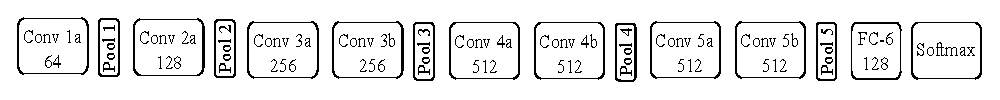
\includegraphics[width=\textwidth]{figures/3D_CNN.eps}}
	\caption[Proposed 3D-CNN for video angle identification]
	{Proposed 3D-CNN for view angle identification. Last 3 layers of a pretrained C3D~\cite{Tran_15} network has been replaced by a fully connected layer of 128 neurons followed a final softmax layer of 11 neurons to classify 11 different walking directions of CASIA B dataset. \label{fig:3D_CNN}
	}
\end{figure}

\subsection{Network for View Angle Identification}
Successful transfer learning within or across different domain of interest leads to significant improvement in performance due to the amount of jointly learning representations in a shared feature space. In our work, we used a pretrained C3D model and fine-tuned it for our 3D Convolutional network to determine the view angle from gait videos. Fig.~\ref{fig:3D_CNN} shows our proposed 3D convolutional network. 

C3D network is composed of 8 convolutional layers, 5 pooling layers, 2 fully-connected layers, followed by a softmax layer at the end. All the 3D convolution kernels are $3\times3\times3$ with stride 1 in both spatial and temporal dimensions. We removed the last 3 layer from the model and then added a fully connected layer of 128 neurons and a dropout layer of 0.5 to avoid overfitting. Finally, a softmax layer of 11 neuron has been added to classify any given videos into 11 different viewing angles. 

The proposed method for our view angle identification is illustrated in Figure~\ref{fig:view_angle_identification}. The input of the network was a clip of 16 consecutive frame which was preprocessed and resized to $112\times112$ to feed into a  3D-CNN network. We used {\textit {majority voting scheme}} to process the output to predict the view angle similar to section~\ref{subsec_post_process}, i.e. the angle that receives the highest number of votes over all clips are referred as predicted angle of the video.



\subsection{Two-Stage Network for Multi-View Gait Recognition}
\begin{figure}[t]
	\centering {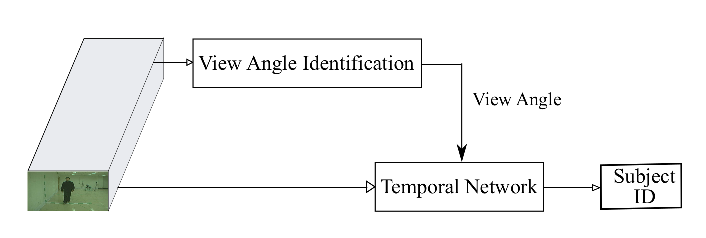
\includegraphics[width=0.8\textwidth]{figures/two-stage_network.eps}}
	\caption[Poposed two-stage network for multi-view gait recognition.]
	{Poposed two-stage network for multi-view gait recognition.\label{fig:two-stage_network}
	}
\end{figure}


\subsection{Training Details}
We employed CASIA B gait dataset~\cite{Yu_06} to train our model. We trained the network using 4 normal walking sequences of 100 subjects in gallery set of CASIA B as described in Table~\ref{table:caisab_setup}. Our network was trained with a 12 batch size with an initial learning rate ${10^{-3}}$ for 70 epochs. Table~\ref{table:summary_3dcnn} summarizes all of the hyperparameters setting of our proposed network.


